
% Default to the notebook output style

    


% Inherit from the specified cell style.




    
\documentclass[11pt]{article}

    
    
    \usepackage[T1]{fontenc}
    % Nicer default font (+ math font) than Computer Modern for most use cases
    \usepackage{mathpazo}

    % Basic figure setup, for now with no caption control since it's done
    % automatically by Pandoc (which extracts ![](path) syntax from Markdown).
    \usepackage{graphicx}
    \usepackage{float}
    % We will generate all images so they have a width \maxwidth. This means
    % that they will get their normal width if they fit onto the page, but
    % are scaled down if they would overflow the margins.
    \makeatletter
    \def\maxwidth{\ifdim\Gin@nat@width>\linewidth\linewidth
    \else\Gin@nat@width\fi}
    \makeatother
    \let\Oldincludegraphics\includegraphics
    % Set max figure width to be 80% of text width, for now hardcoded.
    \renewcommand{\includegraphics}[1]{\Oldincludegraphics[width=.8\maxwidth]{#1}}
    % Ensure that by default, figures have no caption (until we provide a
    % proper Figure object with a Caption API and a way to capture that
    % in the conversion process - todo).
    \usepackage{caption}
    \DeclareCaptionLabelFormat{nolabel}{}
    \captionsetup{labelformat=nolabel}

    \usepackage{adjustbox} % Used to constrain images to a maximum size 
    \usepackage{xcolor} % Allow colors to be defined
    \usepackage{enumerate} % Needed for markdown enumerations to work
    \usepackage{geometry} % Used to adjust the document margins
    \usepackage{amsmath} % Equations
    \usepackage{amssymb} % Equations
    \usepackage{textcomp} % defines textquotesingle
    % Hack from http://tex.stackexchange.com/a/47451/13684:
    \AtBeginDocument{%
        \def\PYZsq{\textquotesingle}% Upright quotes in Pygmentized code
    }
    \usepackage{upquote} % Upright quotes for verbatim code
    \usepackage{eurosym} % defines \euro
    \usepackage[mathletters]{ucs} % Extended unicode (utf-8) support
    \usepackage[utf8x]{inputenc} % Allow utf-8 characters in the tex document
    \usepackage{fancyvrb} % verbatim replacement that allows latex
    \usepackage{grffile} % extends the file name processing of package graphics 
                         % to support a larger range 
    % The hyperref package gives us a pdf with properly built
    % internal navigation ('pdf bookmarks' for the table of contents,
    % internal cross-reference links, web links for URLs, etc.)
    \usepackage{hyperref}
    \usepackage{longtable} % longtable support required by pandoc >1.10
    \usepackage{booktabs}  % table support for pandoc > 1.12.2
    \usepackage[inline]{enumitem} % IRkernel/repr support (it uses the enumerate* environment)
    \usepackage[normalem]{ulem} % ulem is needed to support strikethroughs (\sout)
                                % normalem makes italics be italics, not underlines
    \usepackage{mathrsfs}
    

    
    
    % Colors for the hyperref package
    \definecolor{urlcolor}{rgb}{0,.145,.698}
    \definecolor{linkcolor}{rgb}{.71,0.21,0.01}
    \definecolor{citecolor}{rgb}{.12,.54,.11}

    % ANSI colors
    \definecolor{ansi-black}{HTML}{3E424D}
    \definecolor{ansi-black-intense}{HTML}{282C36}
    \definecolor{ansi-red}{HTML}{E75C58}
    \definecolor{ansi-red-intense}{HTML}{B22B31}
    \definecolor{ansi-green}{HTML}{00A250}
    \definecolor{ansi-green-intense}{HTML}{007427}
    \definecolor{ansi-yellow}{HTML}{DDB62B}
    \definecolor{ansi-yellow-intense}{HTML}{B27D12}
    \definecolor{ansi-blue}{HTML}{208FFB}
    \definecolor{ansi-blue-intense}{HTML}{0065CA}
    \definecolor{ansi-magenta}{HTML}{D160C4}
    \definecolor{ansi-magenta-intense}{HTML}{A03196}
    \definecolor{ansi-cyan}{HTML}{60C6C8}
    \definecolor{ansi-cyan-intense}{HTML}{258F8F}
    \definecolor{ansi-white}{HTML}{C5C1B4}
    \definecolor{ansi-white-intense}{HTML}{A1A6B2}
    \definecolor{ansi-default-inverse-fg}{HTML}{FFFFFF}
    \definecolor{ansi-default-inverse-bg}{HTML}{000000}

    % commands and environments needed by pandoc snippets
    % extracted from the output of `pandoc -s`
    \providecommand{\tightlist}{%
      \setlength{\itemsep}{0pt}\setlength{\parskip}{0pt}}
    \DefineVerbatimEnvironment{Highlighting}{Verbatim}{commandchars=\\\{\}}
    % Add ',fontsize=\small' for more characters per line
    \newenvironment{Shaded}{}{}
    \newcommand{\KeywordTok}[1]{\textcolor[rgb]{0.00,0.44,0.13}{\textbf{{#1}}}}
    \newcommand{\DataTypeTok}[1]{\textcolor[rgb]{0.56,0.13,0.00}{{#1}}}
    \newcommand{\DecValTok}[1]{\textcolor[rgb]{0.25,0.63,0.44}{{#1}}}
    \newcommand{\BaseNTok}[1]{\textcolor[rgb]{0.25,0.63,0.44}{{#1}}}
    \newcommand{\FloatTok}[1]{\textcolor[rgb]{0.25,0.63,0.44}{{#1}}}
    \newcommand{\CharTok}[1]{\textcolor[rgb]{0.25,0.44,0.63}{{#1}}}
    \newcommand{\StringTok}[1]{\textcolor[rgb]{0.25,0.44,0.63}{{#1}}}
    \newcommand{\CommentTok}[1]{\textcolor[rgb]{0.38,0.63,0.69}{\textit{{#1}}}}
    \newcommand{\OtherTok}[1]{\textcolor[rgb]{0.00,0.44,0.13}{{#1}}}
    \newcommand{\AlertTok}[1]{\textcolor[rgb]{1.00,0.00,0.00}{\textbf{{#1}}}}
    \newcommand{\FunctionTok}[1]{\textcolor[rgb]{0.02,0.16,0.49}{{#1}}}
    \newcommand{\RegionMarkerTok}[1]{{#1}}
    \newcommand{\ErrorTok}[1]{\textcolor[rgb]{1.00,0.00,0.00}{\textbf{{#1}}}}
    \newcommand{\NormalTok}[1]{{#1}}
    
    % Additional commands for more recent versions of Pandoc
    \newcommand{\ConstantTok}[1]{\textcolor[rgb]{0.53,0.00,0.00}{{#1}}}
    \newcommand{\SpecialCharTok}[1]{\textcolor[rgb]{0.25,0.44,0.63}{{#1}}}
    \newcommand{\VerbatimStringTok}[1]{\textcolor[rgb]{0.25,0.44,0.63}{{#1}}}
    \newcommand{\SpecialStringTok}[1]{\textcolor[rgb]{0.73,0.40,0.53}{{#1}}}
    \newcommand{\ImportTok}[1]{{#1}}
    \newcommand{\DocumentationTok}[1]{\textcolor[rgb]{0.73,0.13,0.13}{\textit{{#1}}}}
    \newcommand{\AnnotationTok}[1]{\textcolor[rgb]{0.38,0.63,0.69}{\textbf{\textit{{#1}}}}}
    \newcommand{\CommentVarTok}[1]{\textcolor[rgb]{0.38,0.63,0.69}{\textbf{\textit{{#1}}}}}
    \newcommand{\VariableTok}[1]{\textcolor[rgb]{0.10,0.09,0.49}{{#1}}}
    \newcommand{\ControlFlowTok}[1]{\textcolor[rgb]{0.00,0.44,0.13}{\textbf{{#1}}}}
    \newcommand{\OperatorTok}[1]{\textcolor[rgb]{0.40,0.40,0.40}{{#1}}}
    \newcommand{\BuiltInTok}[1]{{#1}}
    \newcommand{\ExtensionTok}[1]{{#1}}
    \newcommand{\PreprocessorTok}[1]{\textcolor[rgb]{0.74,0.48,0.00}{{#1}}}
    \newcommand{\AttributeTok}[1]{\textcolor[rgb]{0.49,0.56,0.16}{{#1}}}
    \newcommand{\InformationTok}[1]{\textcolor[rgb]{0.38,0.63,0.69}{\textbf{\textit{{#1}}}}}
    \newcommand{\WarningTok}[1]{\textcolor[rgb]{0.38,0.63,0.69}{\textbf{\textit{{#1}}}}}
    
    
    % Define a nice break command that doesn't care if a line doesn't already
    % exist.
    \def\br{\hspace*{\fill} \\* }
    % Math Jax compatibility definitions
    \def\gt{>}
    \def\lt{<}
    \let\Oldtex\TeX
    \let\Oldlatex\LaTeX
    \renewcommand{\TeX}{\textrm{\Oldtex}}
    \renewcommand{\LaTeX}{\textrm{\Oldlatex}}
    % Document parameters
    % Document title
    \title{PD1}
    
    \author{Jiarong Ye, Yuan Meng}
    
    
    
    
    

    % Pygments definitions
    
\makeatletter
\def\PY@reset{\let\PY@it=\relax \let\PY@bf=\relax%
    \let\PY@ul=\relax \let\PY@tc=\relax%
    \let\PY@bc=\relax \let\PY@ff=\relax}
\def\PY@tok#1{\csname PY@tok@#1\endcsname}
\def\PY@toks#1+{\ifx\relax#1\empty\else%
    \PY@tok{#1}\expandafter\PY@toks\fi}
\def\PY@do#1{\PY@bc{\PY@tc{\PY@ul{%
    \PY@it{\PY@bf{\PY@ff{#1}}}}}}}
\def\PY#1#2{\PY@reset\PY@toks#1+\relax+\PY@do{#2}}

\expandafter\def\csname PY@tok@w\endcsname{\def\PY@tc##1{\textcolor[rgb]{0.73,0.73,0.73}{##1}}}
\expandafter\def\csname PY@tok@c\endcsname{\let\PY@it=\textit\def\PY@tc##1{\textcolor[rgb]{0.25,0.50,0.50}{##1}}}
\expandafter\def\csname PY@tok@cp\endcsname{\def\PY@tc##1{\textcolor[rgb]{0.74,0.48,0.00}{##1}}}
\expandafter\def\csname PY@tok@k\endcsname{\let\PY@bf=\textbf\def\PY@tc##1{\textcolor[rgb]{0.00,0.50,0.00}{##1}}}
\expandafter\def\csname PY@tok@kp\endcsname{\def\PY@tc##1{\textcolor[rgb]{0.00,0.50,0.00}{##1}}}
\expandafter\def\csname PY@tok@kt\endcsname{\def\PY@tc##1{\textcolor[rgb]{0.69,0.00,0.25}{##1}}}
\expandafter\def\csname PY@tok@o\endcsname{\def\PY@tc##1{\textcolor[rgb]{0.40,0.40,0.40}{##1}}}
\expandafter\def\csname PY@tok@ow\endcsname{\let\PY@bf=\textbf\def\PY@tc##1{\textcolor[rgb]{0.67,0.13,1.00}{##1}}}
\expandafter\def\csname PY@tok@nb\endcsname{\def\PY@tc##1{\textcolor[rgb]{0.00,0.50,0.00}{##1}}}
\expandafter\def\csname PY@tok@nf\endcsname{\def\PY@tc##1{\textcolor[rgb]{0.00,0.00,1.00}{##1}}}
\expandafter\def\csname PY@tok@nc\endcsname{\let\PY@bf=\textbf\def\PY@tc##1{\textcolor[rgb]{0.00,0.00,1.00}{##1}}}
\expandafter\def\csname PY@tok@nn\endcsname{\let\PY@bf=\textbf\def\PY@tc##1{\textcolor[rgb]{0.00,0.00,1.00}{##1}}}
\expandafter\def\csname PY@tok@ne\endcsname{\let\PY@bf=\textbf\def\PY@tc##1{\textcolor[rgb]{0.82,0.25,0.23}{##1}}}
\expandafter\def\csname PY@tok@nv\endcsname{\def\PY@tc##1{\textcolor[rgb]{0.10,0.09,0.49}{##1}}}
\expandafter\def\csname PY@tok@no\endcsname{\def\PY@tc##1{\textcolor[rgb]{0.53,0.00,0.00}{##1}}}
\expandafter\def\csname PY@tok@nl\endcsname{\def\PY@tc##1{\textcolor[rgb]{0.63,0.63,0.00}{##1}}}
\expandafter\def\csname PY@tok@ni\endcsname{\let\PY@bf=\textbf\def\PY@tc##1{\textcolor[rgb]{0.60,0.60,0.60}{##1}}}
\expandafter\def\csname PY@tok@na\endcsname{\def\PY@tc##1{\textcolor[rgb]{0.49,0.56,0.16}{##1}}}
\expandafter\def\csname PY@tok@nt\endcsname{\let\PY@bf=\textbf\def\PY@tc##1{\textcolor[rgb]{0.00,0.50,0.00}{##1}}}
\expandafter\def\csname PY@tok@nd\endcsname{\def\PY@tc##1{\textcolor[rgb]{0.67,0.13,1.00}{##1}}}
\expandafter\def\csname PY@tok@s\endcsname{\def\PY@tc##1{\textcolor[rgb]{0.73,0.13,0.13}{##1}}}
\expandafter\def\csname PY@tok@sd\endcsname{\let\PY@it=\textit\def\PY@tc##1{\textcolor[rgb]{0.73,0.13,0.13}{##1}}}
\expandafter\def\csname PY@tok@si\endcsname{\let\PY@bf=\textbf\def\PY@tc##1{\textcolor[rgb]{0.73,0.40,0.53}{##1}}}
\expandafter\def\csname PY@tok@se\endcsname{\let\PY@bf=\textbf\def\PY@tc##1{\textcolor[rgb]{0.73,0.40,0.13}{##1}}}
\expandafter\def\csname PY@tok@sr\endcsname{\def\PY@tc##1{\textcolor[rgb]{0.73,0.40,0.53}{##1}}}
\expandafter\def\csname PY@tok@ss\endcsname{\def\PY@tc##1{\textcolor[rgb]{0.10,0.09,0.49}{##1}}}
\expandafter\def\csname PY@tok@sx\endcsname{\def\PY@tc##1{\textcolor[rgb]{0.00,0.50,0.00}{##1}}}
\expandafter\def\csname PY@tok@m\endcsname{\def\PY@tc##1{\textcolor[rgb]{0.40,0.40,0.40}{##1}}}
\expandafter\def\csname PY@tok@gh\endcsname{\let\PY@bf=\textbf\def\PY@tc##1{\textcolor[rgb]{0.00,0.00,0.50}{##1}}}
\expandafter\def\csname PY@tok@gu\endcsname{\let\PY@bf=\textbf\def\PY@tc##1{\textcolor[rgb]{0.50,0.00,0.50}{##1}}}
\expandafter\def\csname PY@tok@gd\endcsname{\def\PY@tc##1{\textcolor[rgb]{0.63,0.00,0.00}{##1}}}
\expandafter\def\csname PY@tok@gi\endcsname{\def\PY@tc##1{\textcolor[rgb]{0.00,0.63,0.00}{##1}}}
\expandafter\def\csname PY@tok@gr\endcsname{\def\PY@tc##1{\textcolor[rgb]{1.00,0.00,0.00}{##1}}}
\expandafter\def\csname PY@tok@ge\endcsname{\let\PY@it=\textit}
\expandafter\def\csname PY@tok@gs\endcsname{\let\PY@bf=\textbf}
\expandafter\def\csname PY@tok@gp\endcsname{\let\PY@bf=\textbf\def\PY@tc##1{\textcolor[rgb]{0.00,0.00,0.50}{##1}}}
\expandafter\def\csname PY@tok@go\endcsname{\def\PY@tc##1{\textcolor[rgb]{0.53,0.53,0.53}{##1}}}
\expandafter\def\csname PY@tok@gt\endcsname{\def\PY@tc##1{\textcolor[rgb]{0.00,0.27,0.87}{##1}}}
\expandafter\def\csname PY@tok@err\endcsname{\def\PY@bc##1{\setlength{\fboxsep}{0pt}\fcolorbox[rgb]{1.00,0.00,0.00}{1,1,1}{\strut ##1}}}
\expandafter\def\csname PY@tok@kc\endcsname{\let\PY@bf=\textbf\def\PY@tc##1{\textcolor[rgb]{0.00,0.50,0.00}{##1}}}
\expandafter\def\csname PY@tok@kd\endcsname{\let\PY@bf=\textbf\def\PY@tc##1{\textcolor[rgb]{0.00,0.50,0.00}{##1}}}
\expandafter\def\csname PY@tok@kn\endcsname{\let\PY@bf=\textbf\def\PY@tc##1{\textcolor[rgb]{0.00,0.50,0.00}{##1}}}
\expandafter\def\csname PY@tok@kr\endcsname{\let\PY@bf=\textbf\def\PY@tc##1{\textcolor[rgb]{0.00,0.50,0.00}{##1}}}
\expandafter\def\csname PY@tok@bp\endcsname{\def\PY@tc##1{\textcolor[rgb]{0.00,0.50,0.00}{##1}}}
\expandafter\def\csname PY@tok@fm\endcsname{\def\PY@tc##1{\textcolor[rgb]{0.00,0.00,1.00}{##1}}}
\expandafter\def\csname PY@tok@vc\endcsname{\def\PY@tc##1{\textcolor[rgb]{0.10,0.09,0.49}{##1}}}
\expandafter\def\csname PY@tok@vg\endcsname{\def\PY@tc##1{\textcolor[rgb]{0.10,0.09,0.49}{##1}}}
\expandafter\def\csname PY@tok@vi\endcsname{\def\PY@tc##1{\textcolor[rgb]{0.10,0.09,0.49}{##1}}}
\expandafter\def\csname PY@tok@vm\endcsname{\def\PY@tc##1{\textcolor[rgb]{0.10,0.09,0.49}{##1}}}
\expandafter\def\csname PY@tok@sa\endcsname{\def\PY@tc##1{\textcolor[rgb]{0.73,0.13,0.13}{##1}}}
\expandafter\def\csname PY@tok@sb\endcsname{\def\PY@tc##1{\textcolor[rgb]{0.73,0.13,0.13}{##1}}}
\expandafter\def\csname PY@tok@sc\endcsname{\def\PY@tc##1{\textcolor[rgb]{0.73,0.13,0.13}{##1}}}
\expandafter\def\csname PY@tok@dl\endcsname{\def\PY@tc##1{\textcolor[rgb]{0.73,0.13,0.13}{##1}}}
\expandafter\def\csname PY@tok@s2\endcsname{\def\PY@tc##1{\textcolor[rgb]{0.73,0.13,0.13}{##1}}}
\expandafter\def\csname PY@tok@sh\endcsname{\def\PY@tc##1{\textcolor[rgb]{0.73,0.13,0.13}{##1}}}
\expandafter\def\csname PY@tok@s1\endcsname{\def\PY@tc##1{\textcolor[rgb]{0.73,0.13,0.13}{##1}}}
\expandafter\def\csname PY@tok@mb\endcsname{\def\PY@tc##1{\textcolor[rgb]{0.40,0.40,0.40}{##1}}}
\expandafter\def\csname PY@tok@mf\endcsname{\def\PY@tc##1{\textcolor[rgb]{0.40,0.40,0.40}{##1}}}
\expandafter\def\csname PY@tok@mh\endcsname{\def\PY@tc##1{\textcolor[rgb]{0.40,0.40,0.40}{##1}}}
\expandafter\def\csname PY@tok@mi\endcsname{\def\PY@tc##1{\textcolor[rgb]{0.40,0.40,0.40}{##1}}}
\expandafter\def\csname PY@tok@il\endcsname{\def\PY@tc##1{\textcolor[rgb]{0.40,0.40,0.40}{##1}}}
\expandafter\def\csname PY@tok@mo\endcsname{\def\PY@tc##1{\textcolor[rgb]{0.40,0.40,0.40}{##1}}}
\expandafter\def\csname PY@tok@ch\endcsname{\let\PY@it=\textit\def\PY@tc##1{\textcolor[rgb]{0.25,0.50,0.50}{##1}}}
\expandafter\def\csname PY@tok@cm\endcsname{\let\PY@it=\textit\def\PY@tc##1{\textcolor[rgb]{0.25,0.50,0.50}{##1}}}
\expandafter\def\csname PY@tok@cpf\endcsname{\let\PY@it=\textit\def\PY@tc##1{\textcolor[rgb]{0.25,0.50,0.50}{##1}}}
\expandafter\def\csname PY@tok@c1\endcsname{\let\PY@it=\textit\def\PY@tc##1{\textcolor[rgb]{0.25,0.50,0.50}{##1}}}
\expandafter\def\csname PY@tok@cs\endcsname{\let\PY@it=\textit\def\PY@tc##1{\textcolor[rgb]{0.25,0.50,0.50}{##1}}}

\def\PYZbs{\char`\\}
\def\PYZus{\char`\_}
\def\PYZob{\char`\{}
\def\PYZcb{\char`\}}
\def\PYZca{\char`\^}
\def\PYZam{\char`\&}
\def\PYZlt{\char`\<}
\def\PYZgt{\char`\>}
\def\PYZsh{\char`\#}
\def\PYZpc{\char`\%}
\def\PYZdl{\char`\$}
\def\PYZhy{\char`\-}
\def\PYZsq{\char`\'}
\def\PYZdq{\char`\"}
\def\PYZti{\char`\~}
% for compatibility with earlier versions
\def\PYZat{@}
\def\PYZlb{[}
\def\PYZrb{]}
\makeatother


    % Exact colors from NB
    \definecolor{incolor}{rgb}{0.0, 0.0, 0.5}
    \definecolor{outcolor}{rgb}{0.545, 0.0, 0.0}



    
    % Prevent overflowing lines due to hard-to-break entities
    \sloppy 
    % Setup hyperref package
    \hypersetup{
      breaklinks=true,  % so long urls are correctly broken across lines
      colorlinks=true,
      urlcolor=urlcolor,
      linkcolor=linkcolor,
      citecolor=citecolor,
      }
    % Slightly bigger margins than the latex defaults
    
    \geometry{verbose,tmargin=1in,bmargin=1in,lmargin=1in,rmargin=1in}
    
    

    \begin{document}
    
    
    \maketitle
    
    

    
    \subsubsection*{import packages}\label{import-packages}

    \begin{Verbatim}[commandchars=\\\{\}]
{\color{incolor}In [{\color{incolor}205}]:} \PY{k+kn}{import} \PY{n+nn}{datascience} \PY{k}{as} \PY{n+nn}{ds}
          \PY{k+kn}{from} \PY{n+nn}{datascience} \PY{k}{import} \PY{o}{*}
          \PY{k+kn}{import} \PY{n+nn}{numpy} \PY{k}{as} \PY{n+nn}{np}
          \PY{k+kn}{from} \PY{n+nn}{graphviz} \PY{k}{import} \PY{n}{Source}
          \PY{k+kn}{import} \PY{n+nn}{pandas} \PY{k}{as} \PY{n+nn}{pd}
          \PY{k+kn}{import} \PY{n+nn}{seaborn} \PY{k}{as} \PY{n+nn}{sns}
          \PY{k+kn}{from} \PY{n+nn}{sklearn}\PY{n+nn}{.}\PY{n+nn}{pipeline} \PY{k}{import} \PY{n}{Pipeline}
          \PY{k+kn}{from} \PY{n+nn}{sklearn}\PY{n+nn}{.}\PY{n+nn}{feature\PYZus{}extraction}\PY{n+nn}{.}\PY{n+nn}{text} \PY{k}{import} \PY{n}{CountVectorizer}\PY{p}{,} \PY{n}{TfidfTransformer}
          \PY{k+kn}{from} \PY{n+nn}{sklearn}\PY{n+nn}{.}\PY{n+nn}{tree} \PY{k}{import} \PY{n}{DecisionTreeClassifier}
          \PY{k+kn}{from} \PY{n+nn}{sklearn}\PY{n+nn}{.}\PY{n+nn}{ensemble} \PY{k}{import} \PY{n}{RandomForestClassifier}
          \PY{k+kn}{from} \PY{n+nn}{sklearn} \PY{k}{import} \PY{n}{tree}
          \PY{k+kn}{from} \PY{n+nn}{sklearn}\PY{n+nn}{.}\PY{n+nn}{metrics} \PY{k}{import} \PY{n}{confusion\PYZus{}matrix}\PY{p}{,} \PY{n}{precision\PYZus{}score}\PY{p}{,} \PY{n}{recall\PYZus{}score}\PY{p}{,} \PY{n}{f1\PYZus{}score}\PY{p}{,}
          				 \PY{n}{accuracy\PYZus{}score}\PY{p}{,} \PY{n}{classification\PYZus{}report}
          \PY{k+kn}{import} \PY{n+nn}{matplotlib}\PY{n+nn}{.}\PY{n+nn}{pyplot} \PY{k}{as} \PY{n+nn}{plt}
          \PY{k+kn}{from} \PY{n+nn}{sklearn}\PY{n+nn}{.}\PY{n+nn}{model\PYZus{}selection} \PY{k}{import} \PY{n}{train\PYZus{}test\PYZus{}split}\PY{p}{,} \PY{n}{cross\PYZus{}val\PYZus{}score}\PY{p}{,} \PY{n}{StratifiedKFold}
          \PY{k+kn}{from} \PY{n+nn}{sklearn}\PY{n+nn}{.}\PY{n+nn}{externals} \PY{k}{import} \PY{n}{joblib}
          \PY{o}{\PYZpc{}}\PY{k}{matplotlib} inline
\end{Verbatim}

    \subsubsection*{tweets data loaded into Jupyter Notebook as Table
object}\label{tweets-data-loaded-into-jupyter-notebook-as-table-object}

    \begin{Verbatim}[commandchars=\\\{\}]
{\color{incolor}In [{\color{incolor}26}]:} \PY{n}{df} \PY{o}{=} \PY{n}{ds}\PY{o}{.}\PY{n}{Table}\PY{o}{.}\PY{n}{read\PYZus{}table}\PY{p}{(}\PY{l+s+s1}{\PYZsq{}}\PY{l+s+s1}{Climate1SupportiveLevel.csv}\PY{l+s+s1}{\PYZsq{}}\PY{p}{,} \PY{n}{sep}\PY{o}{=}\PY{l+s+s1}{\PYZsq{}}\PY{l+s+s1}{,}\PY{l+s+s1}{\PYZsq{}}\PY{p}{)}
         \PY{n}{df}
\end{Verbatim}

\begin{Verbatim}[commandchars=\\\{\}]
{\color{outcolor}Out[{\color{outcolor}26}]:} Unnamed: 0 | ID                       | Text                                                         | SupportiveLabel
         0          | 962\_Cleand\_Climate1.csv  | RT @kasserolees: Energy is the \#1 contributer to climate {\ldots} | 1
         1          | 885\_Cleand\_Climate1.csv  | RT @edelman\_barbara: @msnbc why don t you have a climate {\ldots} | 1
         2          | 680\_Cleand\_Climate1.csv  | RT @OtagoGrad: @anthonyfurey @OskieOckham The data doesn {\ldots} | 0
         3          | 1152\_Cleand\_Climate1.csv | The Dow just recorded its 3rd worst day ever. Think @rea {\ldots} | 0
         4          | 731\_Cleand\_Climate1.csv  | RT @SimonBanksHB: I am not going to rule out things base {\ldots} | 0
         5          | 1075\_Cleand\_Climate1.csv | RT @sydneyleemarco: nothing like an 80 degree october da {\ldots} | 1
         6          | 85\_Cleand\_Climate1.csv   | @MerlenesMemos @CNN It's not an act of god. Climate chan {\ldots} | 1
         7          | 654\_Cleand\_Climate1.csv  | RT @MikeLevinCA: When asked about climate change my GOP  {\ldots} | 0
         8          | 916\_Cleand\_Climate1.csv  | RT @gq\_jayq: Bet I got 11 years to run it up https://t.c {\ldots} | 0
         9          | 372\_Cleand\_Climate1.csv  | No they care about the oil billionaires                      | 0
         {\ldots} (1273 rows omitted)
\end{Verbatim}
            
    \subsubsection*{Preprocess}\label{preprocess}

    \begin{Verbatim}[commandchars=\\\{\}]
{\color{incolor}In [{\color{incolor}276}]:} \PY{n}{X} \PY{o}{=} \PY{n+nb}{list}\PY{p}{(}\PY{n}{df}\PY{p}{[}\PY{l+s+s1}{\PYZsq{}}\PY{l+s+s1}{Text}\PY{l+s+s1}{\PYZsq{}}\PY{p}{]}\PY{p}{)}
          \PY{n}{y} \PY{o}{=} \PY{n+nb}{list}\PY{p}{(}\PY{n}{df}\PY{p}{[}\PY{l+s+s1}{\PYZsq{}}\PY{l+s+s1}{SupportiveLabel}\PY{l+s+s1}{\PYZsq{}}\PY{p}{]}\PY{p}{)}
\end{Verbatim}

    \subsubsection*{Check whether the data distribution is
balanced}\label{check-whether-the-data-distribution-is-balanced}

    \begin{Verbatim}[commandchars=\\\{\}]
{\color{incolor}In [{\color{incolor}89}]:} \PY{k}{def} \PY{n+nf}{check}\PY{p}{(}\PY{n}{sentiment}\PY{p}{,} \PY{n}{index}\PY{p}{,} \PY{n}{note}\PY{o}{=}\PY{l+s+s1}{\PYZsq{}}\PY{l+s+s1}{training}\PY{l+s+s1}{\PYZsq{}}\PY{p}{)}\PY{p}{:}
             \PY{k}{if} \PY{n}{sentiment}\PY{o}{==}\PY{l+m+mi}{0}\PY{p}{:}
                 \PY{n}{label} \PY{o}{=} \PY{l+s+s1}{\PYZsq{}}\PY{l+s+s1}{not supportive}\PY{l+s+s1}{\PYZsq{}}
             \PY{k}{else}\PY{p}{:}
                 \PY{n}{label} \PY{o}{=} \PY{l+s+s1}{\PYZsq{}}\PY{l+s+s1}{supportive}\PY{l+s+s1}{\PYZsq{}}
             \PY{n+nb}{print}\PY{p}{(}\PY{l+s+s1}{\PYZsq{}}\PY{l+s+s1}{There are }\PY{l+s+si}{\PYZob{}\PYZcb{}}\PY{l+s+s1}{ }\PY{l+s+s1}{\PYZsq{}}\PY{o}{.}\PY{n}{format}\PY{p}{(}\PY{n}{df}\PY{o}{.}\PY{n}{take}\PY{p}{(}\PY{n}{index}\PY{p}{)}\PY{o}{.}\PY{n}{where}\PY{p}{(}\PY{l+s+s1}{\PYZsq{}}\PY{l+s+s1}{SupportiveLabel}\PY{l+s+s1}{\PYZsq{}}\PY{p}{,} 
                   \PY{n}{are}\PY{o}{.}\PY{n}{equal\PYZus{}to}\PY{p}{(}\PY{n}{sentiment}\PY{p}{)}\PY{p}{)}\PY{o}{.}\PY{n}{size}\PY{p}{[}\PY{l+m+mi}{0}\PY{p}{]}\PY{p}{[}\PY{l+m+mi}{0}\PY{p}{]}\PY{p}{)}\PY{o}{+}\PY{n}{label}\PY{o}{+}\PY{l+s+s1}{\PYZsq{}}\PY{l+s+s1}{ tweets in the }\PY{l+s+s1}{\PYZsq{}}\PY{o}{+}\PY{n}{note}\PY{o}{+}\PY{l+s+s1}{\PYZsq{}}\PY{l+s+s1}{ set.}\PY{l+s+s1}{\PYZsq{}}\PY{p}{)}
\end{Verbatim}

    \paragraph{Model Building}\label{model-building}

    \begin{Verbatim}[commandchars=\\\{\}]
{\color{incolor}In [{\color{incolor}90}]:} \PY{k}{def} \PY{n+nf}{custom\PYZus{}split}\PY{p}{(}\PY{n}{train\PYZus{}index}\PY{p}{,} \PY{n}{test\PYZus{}index}\PY{p}{)}\PY{p}{:}
             \PY{n}{trainingset} \PY{o}{=} \PY{n}{df}\PY{o}{.}\PY{n}{take}\PY{p}{(}\PY{n}{train\PYZus{}index}\PY{p}{)}
             \PY{n}{testingset} \PY{o}{=} \PY{n}{df}\PY{o}{.}\PY{n}{take}\PY{p}{(}\PY{n}{test\PYZus{}index}\PY{p}{)}    
                 
             \PY{n}{X\PYZus{}train}\PY{o}{=} \PY{n+nb}{list}\PY{p}{(}\PY{n}{trainingset}\PY{p}{[}\PY{l+s+s1}{\PYZsq{}}\PY{l+s+s1}{Text}\PY{l+s+s1}{\PYZsq{}}\PY{p}{]}\PY{p}{)}
             \PY{n}{y\PYZus{}train}\PY{o}{=} \PY{n+nb}{list}\PY{p}{(}\PY{n}{trainingset}\PY{p}{[}\PY{l+s+s1}{\PYZsq{}}\PY{l+s+s1}{SupportiveLabel}\PY{l+s+s1}{\PYZsq{}}\PY{p}{]}\PY{p}{)}
             \PY{n}{X\PYZus{}test}\PY{o}{=} \PY{n+nb}{list}\PY{p}{(}\PY{n}{testingset}\PY{p}{[}\PY{l+s+s1}{\PYZsq{}}\PY{l+s+s1}{Text}\PY{l+s+s1}{\PYZsq{}}\PY{p}{]}\PY{p}{)}
             \PY{n}{y\PYZus{}test}\PY{o}{=} \PY{n+nb}{list}\PY{p}{(}\PY{n}{testingset}\PY{p}{[}\PY{l+s+s1}{\PYZsq{}}\PY{l+s+s1}{SupportiveLabel}\PY{l+s+s1}{\PYZsq{}}\PY{p}{]}\PY{p}{)}
             
             \PY{k}{return} \PY{n}{X\PYZus{}train}\PY{p}{,} \PY{n}{X\PYZus{}test}\PY{p}{,} \PY{n}{y\PYZus{}train}\PY{p}{,} \PY{n}{y\PYZus{}test}
\end{Verbatim}

    \subsubsection*{classifier}\label{classifier}

    \begin{Verbatim}[commandchars=\\\{\}]
{\color{incolor}In [{\color{incolor}291}]:} \PY{k}{def} \PY{n+nf}{classifier}\PY{p}{(}\PY{n}{X\PYZus{}train}\PY{p}{,} \PY{n}{y\PYZus{}train}\PY{p}{,} \PY{n}{X\PYZus{}test}\PY{p}{,} \PY{n}{fold}\PY{p}{,} \PY{n}{max\PYZus{}depth}\PY{p}{,} \PY{n}{min\PYZus{}samples\PYZus{}leaf}\PY{p}{)}\PY{p}{:}
              \PY{c+c1}{\PYZsh{} token\PYZus{}pattern=\PYZsq{}(([\PYZsh{}@]|[0\PYZhy{}9]|[a\PYZhy{}z]|[A\PYZhy{}Z])+)\PYZsq{}}
              \PY{n}{clf} \PY{o}{=} \PY{n}{Pipeline}\PY{p}{(}
                  \PY{p}{[}
                      \PY{p}{(}\PY{l+s+s1}{\PYZsq{}}\PY{l+s+s1}{vect}\PY{l+s+s1}{\PYZsq{}}\PY{p}{,} \PY{n}{CountVectorizer}\PY{p}{(}\PY{n}{token\PYZus{}pattern}\PY{o}{=}\PY{l+s+s2}{\PYZdq{}}\PY{l+s+s2}{(?!RT|rt|}\PY{l+s+s2}{\PYZbs{}}\PY{l+s+s2}{d+)[@\PYZsh{}]*[}\PY{l+s+s2}{\PYZbs{}}\PY{l+s+s2}{w}\PY{l+s+se}{\PYZbs{}\PYZsq{}}\PY{l+s+s2}{\PYZus{}\PYZhy{}]}\PY{l+s+s2}{\PYZob{}}\PY{l+s+s2}{2,100\PYZcb{}}\PY{l+s+s2}{\PYZdq{}}\PY{p}{,}
                                               \PY{n}{analyzer} \PY{o}{=} \PY{l+s+s1}{\PYZsq{}}\PY{l+s+s1}{word}\PY{l+s+s1}{\PYZsq{}}\PY{p}{,}
                                               \PY{n}{stop\PYZus{}words}\PY{o}{=}\PY{l+s+s1}{\PYZsq{}}\PY{l+s+s1}{english}\PY{l+s+s1}{\PYZsq{}}\PY{p}{,}
                                               \PY{n}{min\PYZus{}df} \PY{o}{=} \PY{l+m+mi}{3}\PY{p}{)}\PY{p}{)}\PY{p}{,}
                      \PY{p}{(}\PY{l+s+s1}{\PYZsq{}}\PY{l+s+s1}{clf}\PY{l+s+s1}{\PYZsq{}}\PY{p}{,} \PY{n}{DecisionTreeClassifier}\PY{p}{(}\PY{n}{criterion}\PY{o}{=}\PY{l+s+s1}{\PYZsq{}}\PY{l+s+s1}{entropy}\PY{l+s+s1}{\PYZsq{}}\PY{p}{,}
                                                     \PY{n}{random\PYZus{}state} \PY{o}{=} \PY{l+m+mi}{100}\PY{p}{,}
                                                     \PY{n}{max\PYZus{}depth} \PY{o}{=} \PY{n}{max\PYZus{}depth}\PY{p}{,}
                                                     \PY{n}{min\PYZus{}samples\PYZus{}leaf} \PY{o}{=} \PY{n}{min\PYZus{}samples\PYZus{}leaf}\PY{p}{)}\PY{p}{)}
                  \PY{p}{]}\PY{p}{)}
              \PY{n}{clf}\PY{o}{.}\PY{n}{fit}\PY{p}{(}\PY{n}{X\PYZus{}train}\PY{p}{,} \PY{n}{y\PYZus{}train}\PY{p}{)}
              \PY{n}{feature\PYZus{}names} \PY{o}{=} \PY{n}{clf}\PY{o}{.}\PY{n}{named\PYZus{}steps}\PY{p}{[}\PY{l+s+s1}{\PYZsq{}}\PY{l+s+s1}{vect}\PY{l+s+s1}{\PYZsq{}}\PY{p}{]}\PY{o}{.}\PY{n}{get\PYZus{}feature\PYZus{}names}\PY{p}{(}\PY{p}{)}
              \PY{k}{try}\PY{p}{:}
                  \PY{n}{dot\PYZus{}data} \PY{o}{=} \PY{n}{tree}\PY{o}{.}\PY{n}{export\PYZus{}graphviz}\PY{p}{(}\PY{n}{clf}\PY{o}{.}\PY{n}{named\PYZus{}steps}\PY{p}{[}\PY{l+s+s1}{\PYZsq{}}\PY{l+s+s1}{clf}\PY{l+s+s1}{\PYZsq{}}\PY{p}{]}\PY{p}{,} \PY{n}{out\PYZus{}file}\PY{o}{=}\PY{k+kc}{None}\PY{p}{,} 
                                                  \PY{n}{feature\PYZus{}names}\PY{o}{=}\PY{n}{feature\PYZus{}names}\PY{p}{)}
                  \PY{n}{graph} \PY{o}{=} \PY{n}{Source}\PY{p}{(}\PY{n}{dot\PYZus{}data}\PY{p}{)}
                  \PY{n}{graph}\PY{o}{.}\PY{n}{render}\PY{p}{(}\PY{l+s+s1}{\PYZsq{}}\PY{l+s+s1}{ClimateClassifier\PYZhy{}Fold\PYZus{}}\PY{l+s+si}{\PYZob{}\PYZcb{}}\PY{l+s+s1}{\PYZsq{}}\PY{o}{.}\PY{n}{format}\PY{p}{(}\PY{n}{fold}\PY{p}{)}\PY{p}{)}
              \PY{k}{except} \PY{n+ne}{Exception} \PY{k}{as} \PY{n}{e}\PY{p}{:}
                  \PY{n+nb}{print}\PY{p}{(}\PY{n}{e}\PY{p}{)}
              \PY{n}{predicted\PYZus{}y\PYZus{}train} \PY{o}{=} \PY{n}{clf}\PY{o}{.}\PY{n}{predict}\PY{p}{(}\PY{n}{X\PYZus{}train}\PY{p}{)}
              \PY{n}{predicted\PYZus{}y\PYZus{}test} \PY{o}{=} \PY{n}{clf}\PY{o}{.}\PY{n}{predict}\PY{p}{(}\PY{n}{X\PYZus{}test}\PY{p}{)}
              \PY{c+c1}{\PYZsh{} save as pickle}
              \PY{n}{joblib}\PY{o}{.}\PY{n}{dump}\PY{p}{(}\PY{n}{clf}\PY{p}{,} \PY{l+s+s1}{\PYZsq{}}\PY{l+s+s1}{ClimateTeam7PD1.pkl}\PY{l+s+s1}{\PYZsq{}}\PY{p}{)}
              \PY{k}{return} \PY{n}{predicted\PYZus{}y\PYZus{}train}\PY{p}{,} \PY{n}{predicted\PYZus{}y\PYZus{}test}
\end{Verbatim}

    \begin{Verbatim}[commandchars=\\\{\}]
{\color{incolor}In [{\color{incolor}283}]:} \PY{n}{c}\PY{o}{=}\PY{n}{CountVectorizer}\PY{p}{(}\PY{n}{token\PYZus{}pattern}\PY{o}{=}\PY{l+s+s2}{\PYZdq{}}\PY{l+s+s2}{(?!RT|rt|}\PY{l+s+s2}{\PYZbs{}}\PY{l+s+s2}{d+)[@\PYZsh{}]*[}\PY{l+s+s2}{\PYZbs{}}\PY{l+s+s2}{w}\PY{l+s+se}{\PYZbs{}\PYZsq{}}\PY{l+s+s2}{\PYZus{}\PYZhy{}]}\PY{l+s+s2}{\PYZob{}}\PY{l+s+s2}{2,100\PYZcb{}}\PY{l+s+s2}{\PYZdq{}}\PY{p}{,}
                                               \PY{n}{analyzer} \PY{o}{=} \PY{l+s+s1}{\PYZsq{}}\PY{l+s+s1}{word}\PY{l+s+s1}{\PYZsq{}}\PY{p}{,}
                                               \PY{n}{stop\PYZus{}words}\PY{o}{=}\PY{l+s+s1}{\PYZsq{}}\PY{l+s+s1}{english}\PY{l+s+s1}{\PYZsq{}}\PY{p}{,}
                                               \PY{n}{min\PYZus{}df} \PY{o}{=} \PY{l+m+mi}{3}\PY{p}{)}
          \PY{n}{c}\PY{o}{.}\PY{n}{fit}\PY{p}{(}\PY{n}{X}\PY{p}{,} \PY{n}{y}\PY{p}{)}
          \PY{n}{c}\PY{o}{.}\PY{n}{get\PYZus{}feature\PYZus{}names}\PY{p}{(}\PY{p}{)}
\end{Verbatim}

\begin{Verbatim}[commandchars=\\\{\}]
{\color{outcolor}Out[{\color{outcolor}283}]:} ['\#1o5c',
           '\#actonclimate',
           '\#auspol',
           '\#cdnpoli',
           '\#climate',
           '\#climateaction',
           '\#climatebreakdown',
           '\#climatechange',
           '\#climatechangeisreal',
           '\#climateimpactsvic',
           '\#dems',
           '\#emissions',
           '\#energy',
           '\#environment',
           '\#florida',
       		....
\end{Verbatim}
            
    \subsubsection*{evaluation}\label{evaluation}

    \begin{Verbatim}[commandchars=\\\{\}]
{\color{incolor}In [{\color{incolor}295}]:} \PY{k}{def} \PY{n+nf}{eval\PYZus{}results}\PY{p}{(}\PY{n}{predicted\PYZus{}y\PYZus{}train}\PY{p}{,} \PY{n}{y\PYZus{}train}\PY{p}{,} \PY{n}{predicted\PYZus{}y\PYZus{}test}\PY{p}{,} \PY{n}{y\PYZus{}test}\PY{p}{)}\PY{p}{:}
              \PY{n}{accuracy\PYZus{}s} \PY{o}{=} \PY{n}{accuracy\PYZus{}score}\PY{p}{(}\PY{n}{y\PYZus{}test}\PY{p}{,} \PY{n}{predicted\PYZus{}y\PYZus{}test}\PY{p}{)}
              \PY{n}{precision\PYZus{}s} \PY{o}{=} \PY{n}{precision\PYZus{}score}\PY{p}{(}\PY{n}{y\PYZus{}test}\PY{p}{,} \PY{n}{predicted\PYZus{}y\PYZus{}test}\PY{p}{)}
              \PY{n}{recall\PYZus{}s} \PY{o}{=} \PY{n}{recall\PYZus{}score}\PY{p}{(}\PY{n}{y\PYZus{}test}\PY{p}{,} \PY{n}{predicted\PYZus{}y\PYZus{}test}\PY{p}{)}
              \PY{n}{f1\PYZus{}s} \PY{o}{=} \PY{n}{f1\PYZus{}score}\PY{p}{(}\PY{n}{y\PYZus{}test}\PY{p}{,} \PY{n}{predicted\PYZus{}y\PYZus{}test}\PY{p}{)}
              \PY{n}{cm\PYZus{}train} \PY{o}{=} \PY{n}{confusion\PYZus{}matrix}\PY{p}{(}\PY{n}{y\PYZus{}train}\PY{p}{,} \PY{n}{predicted\PYZus{}y\PYZus{}train}\PY{p}{)}
              \PY{n}{cm\PYZus{}test} \PY{o}{=} \PY{n}{confusion\PYZus{}matrix}\PY{p}{(}\PY{n}{y\PYZus{}test}\PY{p}{,} \PY{n}{predicted\PYZus{}y\PYZus{}test}\PY{p}{)}  
              
              \PY{n+nb}{print}\PY{p}{(}\PY{l+s+s1}{\PYZsq{}}\PY{l+s+s1}{Accuracy Score:}\PY{l+s+s1}{\PYZsq{}}\PY{p}{,} \PY{n}{accuracy\PYZus{}s}\PY{p}{)}
              \PY{n+nb}{print}\PY{p}{(}\PY{l+s+s2}{\PYZdq{}}\PY{l+s+s2}{Precision Score:}\PY{l+s+s2}{\PYZdq{}}\PY{p}{,} \PY{n}{precision\PYZus{}s}\PY{p}{)}
              \PY{n+nb}{print}\PY{p}{(}\PY{l+s+s2}{\PYZdq{}}\PY{l+s+s2}{Recall Score:}\PY{l+s+s2}{\PYZdq{}}\PY{p}{,} \PY{n}{recall\PYZus{}s}\PY{p}{)}
              \PY{n+nb}{print}\PY{p}{(}\PY{l+s+s2}{\PYZdq{}}\PY{l+s+s2}{f1 Score:}\PY{l+s+s2}{\PYZdq{}}\PY{p}{,} \PY{n}{f1\PYZus{}s}\PY{p}{)}
              \PY{n+nb}{print}\PY{p}{(}\PY{l+s+s1}{\PYZsq{}}\PY{l+s+s1}{confusion\PYZus{}matrix of training set is: }\PY{l+s+se}{\PYZbs{}n}\PY{l+s+s1}{\PYZsq{}}\PY{p}{,} \PY{n}{cm\PYZus{}train}\PY{p}{,} \PY{l+s+s1}{\PYZsq{}}\PY{l+s+se}{\PYZbs{}n}\PY{l+s+s1}{\PYZsq{}}\PY{p}{)}
              \PY{n+nb}{print}\PY{p}{(}\PY{l+s+s1}{\PYZsq{}}\PY{l+s+s1}{confusion\PYZus{}matrix of testing set is: }\PY{l+s+se}{\PYZbs{}n}\PY{l+s+s1}{\PYZsq{}}\PY{p}{,} \PY{n}{cm\PYZus{}test}\PY{p}{,} \PY{l+s+s1}{\PYZsq{}}\PY{l+s+se}{\PYZbs{}n}\PY{l+s+s1}{\PYZsq{}}\PY{p}{)}
              \PY{n+nb}{print}\PY{p}{(}\PY{n}{classification\PYZus{}report}\PY{p}{(}\PY{n}{y\PYZus{}test}\PY{p}{,} \PY{n}{predicted\PYZus{}y\PYZus{}test}\PY{p}{)}\PY{p}{)}
              
              \PY{n}{classes} \PY{o}{=} \PY{p}{[}\PY{l+s+s1}{\PYZsq{}}\PY{l+s+s1}{not supportive}\PY{l+s+s1}{\PYZsq{}}\PY{p}{,} \PY{l+s+s1}{\PYZsq{}}\PY{l+s+s1}{supportive}\PY{l+s+s1}{\PYZsq{}}\PY{p}{]}
              \PY{n}{sns}\PY{o}{.}\PY{n}{heatmap}\PY{p}{(}\PY{n}{cm\PYZus{}train}\PY{p}{,} \PY{n}{annot}\PY{o}{=}\PY{k+kc}{True}\PY{p}{,} \PY{n}{cmap}\PY{o}{=}\PY{l+s+s1}{\PYZsq{}}\PY{l+s+s1}{Blues}\PY{l+s+s1}{\PYZsq{}}\PY{p}{,} \PY{n}{yticklabels}\PY{o}{=}\PY{n}{classes}\PY{p}{,}
              						 \PY{n}{xticklabels}\PY{o}{=}\PY{n}{classes}\PY{p}{)}
              \PY{n}{plt}\PY{o}{.}\PY{n}{title}\PY{p}{(}\PY{l+s+s1}{\PYZsq{}}\PY{l+s+s1}{confusion matrix of training set}\PY{l+s+s1}{\PYZsq{}}\PY{p}{)}
              \PY{n}{plt}\PY{o}{.}\PY{n}{show}\PY{p}{(}\PY{p}{)}
              \PY{n}{sns}\PY{o}{.}\PY{n}{heatmap}\PY{p}{(}\PY{n}{cm\PYZus{}test}\PY{p}{,} \PY{n}{annot}\PY{o}{=}\PY{k+kc}{True}\PY{p}{,} \PY{n}{cmap}\PY{o}{=}\PY{l+s+s1}{\PYZsq{}}\PY{l+s+s1}{Blues}\PY{l+s+s1}{\PYZsq{}}\PY{p}{,} \PY{n}{yticklabels}\PY{o}{=}\PY{n}{classes}\PY{p}{,}
              						 \PY{n}{xticklabels}\PY{o}{=}\PY{n}{classes}\PY{p}{)}
              \PY{n}{plt}\PY{o}{.}\PY{n}{title}\PY{p}{(}\PY{l+s+s1}{\PYZsq{}}\PY{l+s+s1}{confusion matrix of testing set}\PY{l+s+s1}{\PYZsq{}}\PY{p}{)}
              \PY{n}{plt}\PY{o}{.}\PY{n}{show}\PY{p}{(}\PY{p}{)}
              \PY{k}{return} \PY{n}{accuracy\PYZus{}s}\PY{p}{,} \PY{n}{precision\PYZus{}s}\PY{p}{,} \PY{n}{recall\PYZus{}s}\PY{p}{,} \PY{n}{f1\PYZus{}s}
\end{Verbatim}

    \subsubsection*{k-fold}\label{k-fold}

    \begin{Verbatim}[commandchars=\\\{\}]
{\color{incolor}In [{\color{incolor}293}]:} \PY{k}{def} \PY{n+nf}{k\PYZus{}fold\PYZus{}evaluate}\PY{p}{(}\PY{n}{X}\PY{p}{,} \PY{n}{y}\PY{p}{,} \PY{n}{max\PYZus{}depth}\PY{p}{,} \PY{n}{min\PYZus{}samples\PYZus{}leaf}\PY{p}{)}\PY{p}{:}
              \PY{c+c1}{\PYZsh{} initialization}
              \PY{n}{accuracy} \PY{o}{=} \PY{p}{[}\PY{p}{]}
              \PY{n}{precision} \PY{o}{=} \PY{p}{[}\PY{p}{]}
              \PY{n}{recall}\PY{o}{=}\PY{p}{[}\PY{p}{]}
              \PY{n}{f1} \PY{o}{=} \PY{p}{[}\PY{p}{]}
              \PY{n}{fold} \PY{o}{=} \PY{l+m+mi}{1}
              \PY{n}{skf} \PY{o}{=} \PY{n}{StratifiedKFold}\PY{p}{(}\PY{n}{n\PYZus{}splits}\PY{o}{=}\PY{l+m+mi}{5}\PY{p}{,} \PY{n}{random\PYZus{}state}\PY{o}{=}\PY{l+m+mi}{1}\PY{p}{,} \PY{n}{shuffle}\PY{o}{=} \PY{k+kc}{True}\PY{p}{)}
              
              \PY{c+c1}{\PYZsh{} build model and collect results}
              \PY{k}{for} \PY{n}{train\PYZus{}index}\PY{p}{,} \PY{n}{test\PYZus{}index} \PY{o+ow}{in} \PY{n}{skf}\PY{o}{.}\PY{n}{split}\PY{p}{(}\PY{n}{X}\PY{p}{,} \PY{n}{y}\PY{p}{)}\PY{p}{:}
                  \PY{k}{if} \PY{n}{fold}\PY{o}{==}\PY{l+m+mi}{1}\PY{p}{:}
                      \PY{n+nb}{list}\PY{p}{(}\PY{n+nb}{map}\PY{p}{(}\PY{k}{lambda} \PY{n}{x}\PY{p}{:} \PY{n}{check}\PY{p}{(}\PY{n}{x}\PY{p}{,} \PY{n}{train\PYZus{}index}\PY{p}{)}\PY{p}{,} \PY{n+nb}{range}\PY{p}{(}\PY{l+m+mi}{2}\PY{p}{)}\PY{p}{)}\PY{p}{)}
                      \PY{n+nb}{list}\PY{p}{(}\PY{n+nb}{map}\PY{p}{(}\PY{k}{lambda} \PY{n}{x}\PY{p}{:} \PY{n}{check}\PY{p}{(}\PY{n}{x}\PY{p}{,} \PY{n}{test\PYZus{}index}\PY{p}{,} \PY{n}{note}\PY{o}{=}\PY{l+s+s1}{\PYZsq{}}\PY{l+s+s1}{testing}\PY{l+s+s1}{\PYZsq{}}\PY{p}{)}\PY{p}{,} \PY{n+nb}{range}\PY{p}{(}\PY{l+m+mi}{2}\PY{p}{)}\PY{p}{)}\PY{p}{)}
                  
                  \PY{n}{X\PYZus{}train}\PY{p}{,} \PY{n}{X\PYZus{}test}\PY{p}{,} \PY{n}{y\PYZus{}train}\PY{p}{,} \PY{n}{y\PYZus{}test} \PY{o}{=} \PY{n}{custom\PYZus{}split}\PY{p}{(}\PY{n}{train\PYZus{}index}\PY{p}{,} \PY{n}{test\PYZus{}index}\PY{p}{)}
                  
                  \PY{n}{predicted\PYZus{}y\PYZus{}train}\PY{p}{,} \PY{n}{predicted\PYZus{}y\PYZus{}test} \PY{o}{=}
                  			 \PY{n}{classifier}\PY{p}{(}\PY{n}{X\PYZus{}train}\PY{o}{=}\PY{n}{X\PYZus{}train}\PY{p}{,} \PY{n}{y\PYZus{}train}\PY{o}{=}\PY{n}{y\PYZus{}train}\PY{p}{,} 
                                                                    \PY{n}{X\PYZus{}test}\PY{o}{=}\PY{n}{X\PYZus{}test}\PY{p}{,} \PY{n}{fold}\PY{o}{=}\PY{n}{fold}\PY{p}{,}
                                                                    \PY{n}{max\PYZus{}depth} \PY{o}{=} \PY{n}{max\PYZus{}depth}\PY{p}{,}
                                                                    \PY{n}{min\PYZus{}samples\PYZus{}leaf} \PY{o}{=} \PY{n}{min\PYZus{}samples\PYZus{}leaf}\PY{p}{)}
                  
                  \PY{n+nb}{print}\PY{p}{(}\PY{l+s+s1}{\PYZsq{}}\PY{l+s+se}{\PYZbs{}n}\PY{l+s+s1}{Fold: }\PY{l+s+si}{\PYZob{}\PYZcb{}}\PY{l+s+s1}{\PYZsq{}}\PY{o}{.}\PY{n}{format}\PY{p}{(}\PY{n}{fold}\PY{p}{)}\PY{p}{)}
                  \PY{n}{accuracy\PYZus{}s}\PY{p}{,} \PY{n}{precision\PYZus{}s}\PY{p}{,} \PY{n}{recall\PYZus{}s}\PY{p}{,} \PY{n}{f1\PYZus{}s} \PY{o}{=} \PY{n}{eval\PYZus{}results}\PY{p}{(}\PY{n}{predicted\PYZus{}y\PYZus{}train}\PY{p}{,}
                  						 \PY{n}{y\PYZus{}train}\PY{p}{,} \PY{n}{predicted\PYZus{}y\PYZus{}test}\PY{p}{,} \PY{n}{y\PYZus{}test}\PY{p}{)}
                  
                  \PY{n}{accuracy}\PY{o}{.}\PY{n}{append}\PY{p}{(}\PY{n}{accuracy\PYZus{}s}\PY{p}{)}
                  \PY{n}{precision}\PY{o}{.}\PY{n}{append}\PY{p}{(}\PY{n}{precision\PYZus{}s}\PY{p}{)}
                  \PY{n}{recall}\PY{o}{.}\PY{n}{append}\PY{p}{(}\PY{n}{recall\PYZus{}s}\PY{p}{)}
                  \PY{n}{f1}\PY{o}{.}\PY{n}{append}\PY{p}{(}\PY{n}{f1\PYZus{}s}\PY{p}{)}
                  
                  \PY{n}{metrics\PYZus{}df} \PY{o}{=} \PY{n}{pd}\PY{o}{.}\PY{n}{DataFrame}\PY{p}{(}
                              \PY{p}{\PYZob{}}
                                  \PY{l+s+s1}{\PYZsq{}}\PY{l+s+s1}{accuracy}\PY{l+s+s1}{\PYZsq{}}\PY{p}{:} \PY{n}{accuracy}\PY{p}{,}
                                  \PY{l+s+s1}{\PYZsq{}}\PY{l+s+s1}{precision}\PY{l+s+s1}{\PYZsq{}}\PY{p}{:} \PY{n}{precision}\PY{p}{,}
                                  \PY{l+s+s1}{\PYZsq{}}\PY{l+s+s1}{recall}\PY{l+s+s1}{\PYZsq{}}\PY{p}{:}\PY{n}{recall}\PY{p}{,}
                                  \PY{l+s+s1}{\PYZsq{}}\PY{l+s+s1}{f1}\PY{l+s+s1}{\PYZsq{}}\PY{p}{:}\PY{n}{f1}
                              \PY{p}{\PYZcb{}}
                          \PY{p}{)}
                  \PY{n}{fold} \PY{o}{+}\PY{o}{=} \PY{l+m+mi}{1}
              \PY{k}{return} \PY{n}{metrics\PYZus{}df}
\end{Verbatim}

    \subsubsection*{Tasks}\label{tasks}

\begin{enumerate}
\def\labelenumi{\alph{enumi})}
\item
  A description of model parameters you tried and the associated
  Stratified k-fold cross validation results for each model parameter
  choice
\item
  Describe the model parameters you chose and the rationale of your
  decision.
\item
  Double check overfitting risk: Compare the model's confusion matrix
  for training data vs the model's confusion matrix for testing data.
\end{enumerate}

    \begin{Verbatim}[commandchars=\\\{\}]
{\color{incolor}In [{\color{incolor}296}]:} \PY{n}{k\PYZus{}fold\PYZus{}evaluate}\PY{p}{(}\PY{n}{X}\PY{p}{,} \PY{n}{y}\PY{p}{,} \PY{n}{max\PYZus{}depth}\PY{o}{=}\PY{l+m+mi}{5}\PY{p}{,} \PY{n}{min\PYZus{}samples\PYZus{}leaf}\PY{o}{=}\PY{l+m+mi}{2}\PY{p}{)}
\end{Verbatim}

  \

    \begin{Verbatim}[commandchars=\\\{\}]
There are 453 not supportive tweets in the training set.
There are 572 supportive tweets in the training set.
There are 114 not supportive tweets in the testing set.
There are 144 supportive tweets in the testing set.

Fold: 1
Accuracy Score: 0.6472868217054264
Precision Score: 0.6853146853146853
Recall Score: 0.6805555555555556
f1 Score: 0.6829268292682927
confusion\_matrix of training set is: 
 [[268 185]
 [153 419]] 

confusion\_matrix of testing set is: 
 [[69 45]
 [46 98]] 

              precision    recall  f1-score   support

           0       0.60      0.61      0.60       114
           1       0.69      0.68      0.68       144

   micro avg       0.65      0.65      0.65       258
   macro avg       0.64      0.64      0.64       258
weighted avg       0.65      0.65      0.65       258


    \end{Verbatim}

    \begin{center}
    \adjustimage{max size={0.6\linewidth}{0.9\paperheight}}{output_18_2.png}
    \end{center}
    { \hspace*{\fill} \\}
    
    \begin{center}
    \adjustimage{max size={0.6\linewidth}{0.6\paperheight}}{output_18_3.png}
    \end{center}
    { \hspace*{\fill} \\}
    
    \begin{Verbatim}[commandchars=\\\{\}]

Fold: 2
Accuracy Score: 0.6809338521400778
Precision Score: 0.7046979865771812
Recall Score: 0.7342657342657343
f1 Score: 0.7191780821917809
confusion\_matrix of training set is: 
 [[263 190]
 [137 436]] 

confusion\_matrix of testing set is: 
 [[ 70  44]
 [ 38 105]] 

              precision    recall  f1-score   support

           0       0.65      0.61      0.63       114
           1       0.70      0.73      0.72       143

   micro avg       0.68      0.68      0.68       257
   macro avg       0.68      0.67      0.67       257
weighted avg       0.68      0.68      0.68       257


    \end{Verbatim}

    \begin{center}
    \adjustimage{max size={0.6\linewidth}{0.6\paperheight}}{output_18_5.png}
    \end{center}
    { \hspace*{\fill} \\}
    
    \begin{center}
    \adjustimage{max size={0.6\linewidth}{0.6\paperheight}}{output_18_6.png}
    \end{center}
    { \hspace*{\fill} \\}
    
    \begin{Verbatim}[commandchars=\\\{\}]

Fold: 3
Accuracy Score: 0.625
Precision Score: 0.6516129032258065
Recall Score: 0.7062937062937062
f1 Score: 0.6778523489932886
confusion\_matrix of training set is: 
 [[273 181]
 [135 438]] 

confusion\_matrix of testing set is: 
 [[ 59  54]
 [ 42 101]] 

              precision    recall  f1-score   support

           0       0.58      0.52      0.55       113
           1       0.65      0.71      0.68       143

   micro avg       0.62      0.62      0.62       256
   macro avg       0.62      0.61      0.61       256
weighted avg       0.62      0.62      0.62       256


    \end{Verbatim}

    \begin{center}
    \adjustimage{max size={0.6\linewidth}{0.6\paperheight}}{output_18_8.png}
    \end{center}
    { \hspace*{\fill} \\}
    
    \begin{center}
    \adjustimage{max size={0.6\linewidth}{0.6\paperheight}}{output_18_9.png}
    \end{center}
    { \hspace*{\fill} \\}
    
    \begin{Verbatim}[commandchars=\\\{\}]

Fold: 4
Accuracy Score: 0.6015625
Precision Score: 0.6289308176100629
Recall Score: 0.6993006993006993
f1 Score: 0.6622516556291391
confusion\_matrix of training set is: 
 [[275 179]
 [136 437]] 

confusion\_matrix of testing set is: 
 [[ 54  59]
 [ 43 100]] 

              precision    recall  f1-score   support

           0       0.56      0.48      0.51       113
           1       0.63      0.70      0.66       143

   micro avg       0.60      0.60      0.60       256
   macro avg       0.59      0.59      0.59       256
weighted avg       0.60      0.60      0.60       256


    \end{Verbatim}

    \begin{center}
    \adjustimage{max size={0.6\linewidth}{0.6\paperheight}}{output_18_11.png}
    \end{center}
    { \hspace*{\fill} \\}
    
    \begin{center}
    \adjustimage{max size={0.6\linewidth}{0.6\paperheight}}{output_18_12.png}
    \end{center}
    { \hspace*{\fill} \\}
    
    \begin{Verbatim}[commandchars=\\\{\}]

Fold: 5
Accuracy Score: 0.63671875
Precision Score: 0.6488095238095238
Recall Score: 0.7622377622377622
f1 Score: 0.7009646302250804
confusion\_matrix of training set is: 
 [[272 182]
 [137 436]] 

confusion\_matrix of testing set is: 
 [[ 54  59]
 [ 34 109]] 

              precision    recall  f1-score   support

           0       0.61      0.48      0.54       113
           1       0.65      0.76      0.70       143

   micro avg       0.64      0.64      0.64       256
   macro avg       0.63      0.62      0.62       256
weighted avg       0.63      0.64      0.63       256


    \end{Verbatim}

    \begin{center}
    \adjustimage{max size={0.6\linewidth}{0.6\paperheight}}{output_18_14.png}
    \end{center}
    { \hspace*{\fill} \\}
    
    \begin{center}
    \adjustimage{max size={0.6\linewidth}{0.6\paperheight}}{output_18_15.png}
    \end{center}
    { \hspace*{\fill} \\}
    
\begin{Verbatim}[commandchars=\\\{\}]
{\color{outcolor}Out[{\color{outcolor}296}]:}    accuracy  precision    recall        f1
          0  0.647287   0.685315  0.680556  0.682927
          1  0.680934   0.704698  0.734266  0.719178
          2  0.625000   0.651613  0.706294  0.677852
          3  0.601562   0.628931  0.699301  0.662252
          4  0.636719   0.648810  0.762238  0.700965
\end{Verbatim}
            
    \begin{Verbatim}[commandchars=\\\{\}]
{\color{incolor}In [{\color{incolor}297}]:} \PY{n}{k\PYZus{}fold\PYZus{}evaluate}\PY{p}{(}\PY{n}{X}\PY{p}{,} \PY{n}{y}\PY{p}{,} \PY{n}{max\PYZus{}depth}\PY{o}{=}\PY{l+m+mi}{6}\PY{p}{,} \PY{n}{min\PYZus{}samples\PYZus{}leaf}\PY{o}{=}\PY{l+m+mi}{2}\PY{p}{)}
\end{Verbatim}

  

    \begin{Verbatim}[commandchars=\\\{\}]
There are 453 not supportive tweets in the training set.
There are 572 supportive tweets in the training set.
There are 114 not supportive tweets in the testing set.
There are 144 supportive tweets in the testing set.

Fold: 1
Accuracy Score: 0.6434108527131783
Precision Score: 0.678082191780822
Recall Score: 0.6875
f1 Score: 0.6827586206896552
confusion\_matrix of training set is: 
 [[273 180]
 [150 422]] 

confusion\_matrix of testing set is: 
 [[67 47]
 [45 99]] 

              precision    recall  f1-score   support

           0       0.60      0.59      0.59       114
           1       0.68      0.69      0.68       144

   micro avg       0.64      0.64      0.64       258
   macro avg       0.64      0.64      0.64       258
weighted avg       0.64      0.64      0.64       258


    \end{Verbatim}

    \begin{center}
    \adjustimage{max size={0.6\linewidth}{0.6\paperheight}}{output_19_2.png}
    \end{center}
    { \hspace*{\fill} \\}
    
    \begin{center}
    \adjustimage{max size={0.6\linewidth}{0.6\paperheight}}{output_19_3.png}
    \end{center}
    { \hspace*{\fill} \\}
    
    \begin{Verbatim}[commandchars=\\\{\}]

Fold: 2
Accuracy Score: 0.6770428015564203
Precision Score: 0.7027027027027027
Recall Score: 0.7272727272727273
f1 Score: 0.7147766323024054
confusion\_matrix of training set is: 
 [[267 186]
 [133 440]] 

confusion\_matrix of testing set is: 
 [[ 70  44]
 [ 39 104]] 

              precision    recall  f1-score   support

           0       0.64      0.61      0.63       114
           1       0.70      0.73      0.71       143

   micro avg       0.68      0.68      0.68       257
   macro avg       0.67      0.67      0.67       257
weighted avg       0.68      0.68      0.68       257


    \end{Verbatim}

    \begin{center}
    \adjustimage{max size={0.6\linewidth}{0.6\paperheight}}{output_19_5.png}
    \end{center}
    { \hspace*{\fill} \\}
    
    \begin{center}
    \adjustimage{max size={0.6\linewidth}{0.6\paperheight}}{output_19_6.png}
    \end{center}
    { \hspace*{\fill} \\}
    
    \begin{Verbatim}[commandchars=\\\{\}]

Fold: 3
Accuracy Score: 0.61328125
Precision Score: 0.6428571428571429
Recall Score: 0.6923076923076923
f1 Score: 0.6666666666666666
confusion\_matrix of training set is: 
 [[280 174]
 [132 441]] 

confusion\_matrix of testing set is: 
 [[58 55]
 [44 99]] 

              precision    recall  f1-score   support

           0       0.57      0.51      0.54       113
           1       0.64      0.69      0.67       143

   micro avg       0.61      0.61      0.61       256
   macro avg       0.61      0.60      0.60       256
weighted avg       0.61      0.61      0.61       256


    \end{Verbatim}

    \begin{center}
    \adjustimage{max size={0.6\linewidth}{0.6\paperheight}}{output_19_8.png}
    \end{center}
    { \hspace*{\fill} \\}
    
    \begin{center}
    \adjustimage{max size={0.6\linewidth}{0.6\paperheight}}{output_19_9.png}
    \end{center}
    { \hspace*{\fill} \\}
    
    \begin{Verbatim}[commandchars=\\\{\}]

Fold: 4
Accuracy Score: 0.609375
Precision Score: 0.6335403726708074
Recall Score: 0.7132867132867133
f1 Score: 0.6710526315789473
confusion\_matrix of training set is: 
 [[272 182]
 [125 448]] 

confusion\_matrix of testing set is: 
 [[ 54  59]
 [ 41 102]] 

              precision    recall  f1-score   support

           0       0.57      0.48      0.52       113
           1       0.63      0.71      0.67       143

   micro avg       0.61      0.61      0.61       256
   macro avg       0.60      0.60      0.60       256
weighted avg       0.60      0.61      0.60       256


    \end{Verbatim}

    \begin{center}
    \adjustimage{max size={0.6\linewidth}{0.6\paperheight}}{output_19_11.png}
    \end{center}
    { \hspace*{\fill} \\}
    
    \begin{center}
    \adjustimage{max size={0.6\linewidth}{0.6\paperheight}}{output_19_12.png}
    \end{center}
    { \hspace*{\fill} \\}
    
    \begin{Verbatim}[commandchars=\\\{\}]

Fold: 5
Accuracy Score: 0.63671875
Precision Score: 0.6488095238095238
Recall Score: 0.7622377622377622
f1 Score: 0.7009646302250804
confusion\_matrix of training set is: 
 [[278 176]
 [133 440]] 

confusion\_matrix of testing set is: 
 [[ 54  59]
 [ 34 109]] 

              precision    recall  f1-score   support

           0       0.61      0.48      0.54       113
           1       0.65      0.76      0.70       143

   micro avg       0.64      0.64      0.64       256
   macro avg       0.63      0.62      0.62       256
weighted avg       0.63      0.64      0.63       256


    \end{Verbatim}

    \begin{center}
    \adjustimage{max size={0.6\linewidth}{0.6\paperheight}}{output_19_14.png}
    \end{center}
    { \hspace*{\fill} \\}
    
    \begin{center}
    \adjustimage{max size={0.6\linewidth}{0.6\paperheight}}{output_19_15.png}
    \end{center}
    { \hspace*{\fill} \\}
    
\begin{Verbatim}[commandchars=\\\{\}]
{\color{outcolor}Out[{\color{outcolor}297}]:}    accuracy  precision    recall        f1
          0  0.643411   0.678082  0.687500  0.682759
          1  0.677043   0.702703  0.727273  0.714777
          2  0.613281   0.642857  0.692308  0.666667
          3  0.609375   0.633540  0.713287  0.671053
          4  0.636719   0.648810  0.762238  0.700965
\end{Verbatim}
            
    \begin{Verbatim}[commandchars=\\\{\}]
{\color{incolor}In [{\color{incolor}298}]:} \PY{n}{k\PYZus{}fold\PYZus{}evaluate}\PY{p}{(}\PY{n}{X}\PY{p}{,} \PY{n}{y}\PY{p}{,} \PY{n}{max\PYZus{}depth}\PY{o}{=}\PY{l+m+mi}{7}\PY{p}{,} \PY{n}{min\PYZus{}samples\PYZus{}leaf}\PY{o}{=}\PY{l+m+mi}{1}\PY{p}{)}
\end{Verbatim}

  

    \begin{Verbatim}[commandchars=\\\{\}]
There are 453 not supportive tweets in the training set.
There are 572 supportive tweets in the training set.
There are 114 not supportive tweets in the testing set.
There are 144 supportive tweets in the testing set.

Fold: 1
Accuracy Score: 0.6434108527131783
Precision Score: 0.678082191780822
Recall Score: 0.6875
f1 Score: 0.6827586206896552
confusion\_matrix of training set is: 
 [[276 177]
 [136 436]] 

confusion\_matrix of testing set is: 
 [[67 47]
 [45 99]] 

              precision    recall  f1-score   support

           0       0.60      0.59      0.59       114
           1       0.68      0.69      0.68       144

   micro avg       0.64      0.64      0.64       258
   macro avg       0.64      0.64      0.64       258
weighted avg       0.64      0.64      0.64       258


    \end{Verbatim}

    \begin{center}
    \adjustimage{max size={0.6\linewidth}{0.6\paperheight}}{output_20_2.png}
    \end{center}
    { \hspace*{\fill} \\}
    
    \begin{center}
    \adjustimage{max size={0.6\linewidth}{0.6\paperheight}}{output_20_3.png}
    \end{center}
    { \hspace*{\fill} \\}
    
    \begin{Verbatim}[commandchars=\\\{\}]

Fold: 2
Accuracy Score: 0.6809338521400778
Precision Score: 0.7103448275862069
Recall Score: 0.7202797202797203
f1 Score: 0.7152777777777778
confusion\_matrix of training set is: 
 [[280 173]
 [139 434]] 

confusion\_matrix of testing set is: 
 [[ 72  42]
 [ 40 103]] 

              precision    recall  f1-score   support

           0       0.64      0.63      0.64       114
           1       0.71      0.72      0.72       143

   micro avg       0.68      0.68      0.68       257
   macro avg       0.68      0.68      0.68       257
weighted avg       0.68      0.68      0.68       257


    \end{Verbatim}

    \begin{center}
    \adjustimage{max size={0.6\linewidth}{0.6\paperheight}}{output_20_5.png}
    \end{center}
    { \hspace*{\fill} \\}
    
    \begin{center}
    \adjustimage{max size={0.6\linewidth}{0.6\paperheight}}{output_20_6.png}
    \end{center}
    { \hspace*{\fill} \\}
    
    \begin{Verbatim}[commandchars=\\\{\}]

Fold: 3
Accuracy Score: 0.61328125
Precision Score: 0.6447368421052632
Recall Score: 0.6853146853146853
f1 Score: 0.6644067796610169
confusion\_matrix of training set is: 
 [[286 168]
 [126 447]] 

confusion\_matrix of testing set is: 
 [[59 54]
 [45 98]] 

              precision    recall  f1-score   support

           0       0.57      0.52      0.54       113
           1       0.64      0.69      0.66       143

   micro avg       0.61      0.61      0.61       256
   macro avg       0.61      0.60      0.60       256
weighted avg       0.61      0.61      0.61       256


    \end{Verbatim}

    \begin{center}
    \adjustimage{max size={0.6\linewidth}{0.6\paperheight}}{output_20_8.png}
    \end{center}
    { \hspace*{\fill} \\}
    
    \begin{center}
    \adjustimage{max size={0.6\linewidth}{0.6\paperheight}}{output_20_9.png}
    \end{center}
    { \hspace*{\fill} \\}
    
    \begin{Verbatim}[commandchars=\\\{\}]

Fold: 4
Accuracy Score: 0.60546875
Precision Score: 0.63125
Recall Score: 0.7062937062937062
f1 Score: 0.6666666666666665
confusion\_matrix of training set is: 
 [[283 171]
 [122 451]] 

confusion\_matrix of testing set is: 
 [[ 54  59]
 [ 42 101]] 

              precision    recall  f1-score   support

           0       0.56      0.48      0.52       113
           1       0.63      0.71      0.67       143

   micro avg       0.61      0.61      0.61       256
   macro avg       0.60      0.59      0.59       256
weighted avg       0.60      0.61      0.60       256


    \end{Verbatim}

    \begin{center}
    \adjustimage{max size={0.6\linewidth}{0.6\paperheight}}{output_20_11.png}
    \end{center}
    { \hspace*{\fill} \\}
    
    \begin{center}
    \adjustimage{max size={0.6\linewidth}{0.6\paperheight}}{output_20_12.png}
    \end{center}
    { \hspace*{\fill} \\}
    
    \begin{Verbatim}[commandchars=\\\{\}]

Fold: 5
Accuracy Score: 0.6328125
Precision Score: 0.6467065868263473
Recall Score: 0.7552447552447552
f1 Score: 0.6967741935483871
confusion\_matrix of training set is: 
 [[281 173]
 [129 444]] 

confusion\_matrix of testing set is: 
 [[ 54  59]
 [ 35 108]] 

              precision    recall  f1-score   support

           0       0.61      0.48      0.53       113
           1       0.65      0.76      0.70       143

   micro avg       0.63      0.63      0.63       256
   macro avg       0.63      0.62      0.62       256
weighted avg       0.63      0.63      0.63       256


    \end{Verbatim}

    \begin{center}
    \adjustimage{max size={0.6\linewidth}{0.6\paperheight}}{output_20_14.png}
    \end{center}
    { \hspace*{\fill} \\}
    
    \begin{center}
    \adjustimage{max size={0.6\linewidth}{0.6\paperheight}}{output_20_15.png}
    \end{center}
    { \hspace*{\fill} \\}
    
\begin{Verbatim}[commandchars=\\\{\}]
{\color{outcolor}Out[{\color{outcolor}298}]:}    accuracy  precision    recall        f1
          0  0.643411   0.678082  0.687500  0.682759
          1  0.680934   0.710345  0.720280  0.715278
          2  0.613281   0.644737  0.685315  0.664407
          3  0.605469   0.631250  0.706294  0.666667
          4  0.632812   0.646707  0.755245  0.696774
\end{Verbatim}
            
    \section*{\texorpdfstring{chosen parameters:
\texttt{max\_depth=7,\ min\_samples\_leaf=2}}{chosen parameters: max\_depth=7, min\_samples\_leaf=2}}\label{chosen-parameters-max_depth7-min_samples_leaf2}

Because the 5-fold f1 score of max\_depth=7, min\_samples\_leaf=2 are
better.

    \begin{Verbatim}[commandchars=\\\{\}]
{\color{incolor}In [{\color{incolor}301}]:} \PY{n}{k\PYZus{}fold\PYZus{}evaluate}\PY{p}{(}\PY{n}{X}\PY{p}{,} \PY{n}{y}\PY{p}{,} \PY{n}{max\PYZus{}depth}\PY{o}{=}\PY{l+m+mi}{7}\PY{p}{,} \PY{n}{min\PYZus{}samples\PYZus{}leaf}\PY{o}{=}\PY{l+m+mi}{2}\PY{p}{)}
\end{Verbatim}


    \begin{Verbatim}[commandchars=\\\{\}]
There are 453 not supportive tweets in the training set.
There are 572 supportive tweets in the training set.
There are 114 not supportive tweets in the testing set.
There are 144 supportive tweets in the testing set.

Fold: 1
Accuracy Score: 0.6550387596899225
Precision Score: 0.6870748299319728
Recall Score: 0.7013888888888888
f1 Score: 0.6941580756013744
confusion\_matrix of training set is: 
 [[273 180]
 [146 426]] 

confusion\_matrix of testing set is: 
 [[ 68  46]
 [ 43 101]] 

              precision    recall  f1-score   support

           0       0.61      0.60      0.60       114
           1       0.69      0.70      0.69       144

   micro avg       0.66      0.66      0.66       258
   macro avg       0.65      0.65      0.65       258
weighted avg       0.65      0.66      0.65       258


    \end{Verbatim}

    \begin{center}
    \adjustimage{max size={0.6\linewidth}{0.6\paperheight}}{output_22_2.png}
    \end{center}
    { \hspace*{\fill} \\}
    
    \begin{center}
    \adjustimage{max size={0.6\linewidth}{0.6\paperheight}}{output_22_3.png}
    \end{center}
    { \hspace*{\fill} \\}
    
    \begin{Verbatim}[commandchars=\\\{\}]

Fold: 2
Accuracy Score: 0.6770428015564203
Precision Score: 0.7054794520547946
Recall Score: 0.7202797202797203
f1 Score: 0.71280276816609
confusion\_matrix of training set is: 
 [[278 175]
 [139 434]] 

confusion\_matrix of testing set is: 
 [[ 71  43]
 [ 40 103]] 

              precision    recall  f1-score   support

           0       0.64      0.62      0.63       114
           1       0.71      0.72      0.71       143

   micro avg       0.68      0.68      0.68       257
   macro avg       0.67      0.67      0.67       257
weighted avg       0.68      0.68      0.68       257


    \end{Verbatim}

    \begin{center}
    \adjustimage{max size={0.6\linewidth}{0.6\paperheight}}{output_22_5.png}
    \end{center}
    { \hspace*{\fill} \\}
    
    \begin{center}
    \adjustimage{max size={0.6\linewidth}{0.6\paperheight}}{output_22_6.png}
    \end{center}
    { \hspace*{\fill} \\}
    
    \begin{Verbatim}[commandchars=\\\{\}]

Fold: 3
Accuracy Score: 0.62109375
Precision Score: 0.6513157894736842
Recall Score: 0.6923076923076923
f1 Score: 0.6711864406779661
confusion\_matrix of training set is: 
 [[285 169]
 [128 445]] 

confusion\_matrix of testing set is: 
 [[60 53]
 [44 99]] 

              precision    recall  f1-score   support

           0       0.58      0.53      0.55       113
           1       0.65      0.69      0.67       143

   micro avg       0.62      0.62      0.62       256
   macro avg       0.61      0.61      0.61       256
weighted avg       0.62      0.62      0.62       256


    \end{Verbatim}

    \begin{center}
    \adjustimage{max size={0.6\linewidth}{0.6\paperheight}}{output_22_8.png}
    \end{center}
    { \hspace*{\fill} \\}
    
    \begin{center}
    \adjustimage{max size={0.6\linewidth}{0.6\paperheight}}{output_22_9.png}
    \end{center}
    { \hspace*{\fill} \\}
    
    \begin{Verbatim}[commandchars=\\\{\}]

Fold: 4
Accuracy Score: 0.60546875
Precision Score: 0.63125
Recall Score: 0.7062937062937062
f1 Score: 0.6666666666666665
confusion\_matrix of training set is: 
 [[281 173]
 [124 449]] 

confusion\_matrix of testing set is: 
 [[ 54  59]
 [ 42 101]] 

              precision    recall  f1-score   support

           0       0.56      0.48      0.52       113
           1       0.63      0.71      0.67       143

   micro avg       0.61      0.61      0.61       256
   macro avg       0.60      0.59      0.59       256
weighted avg       0.60      0.61      0.60       256


    \end{Verbatim}

    \begin{center}
    \adjustimage{max size={0.6\linewidth}{0.6\paperheight}}{output_22_11.png}
    \end{center}
    { \hspace*{\fill} \\}
    
    \begin{center}
    \adjustimage{max size={0.6\linewidth}{0.6\paperheight}}{output_22_12.png}
    \end{center}
    { \hspace*{\fill} \\}
    
    \begin{Verbatim}[commandchars=\\\{\}]

Fold: 5
Accuracy Score: 0.6328125
Precision Score: 0.6467065868263473
Recall Score: 0.7552447552447552
f1 Score: 0.6967741935483871
confusion\_matrix of training set is: 
 [[280 174]
 [129 444]] 

confusion\_matrix of testing set is: 
 [[ 54  59]
 [ 35 108]] 

              precision    recall  f1-score   support

           0       0.61      0.48      0.53       113
           1       0.65      0.76      0.70       143

   micro avg       0.63      0.63      0.63       256
   macro avg       0.63      0.62      0.62       256
weighted avg       0.63      0.63      0.63       256


    \end{Verbatim}

    \begin{center}
    \adjustimage{max size={0.6\linewidth}{0.6\paperheight}}{output_22_14.png}
    \end{center}
    { \hspace*{\fill} \\}
    
    \begin{center}
    \adjustimage{max size={0.6\linewidth}{0.6\paperheight}}{output_22_15.png}
    \end{center}
    { \hspace*{\fill} \\}
    
\begin{Verbatim}[commandchars=\\\{\}]
{\color{outcolor}Out[{\color{outcolor}301}]:}    accuracy  precision    recall        f1
          0  0.655039   0.687075  0.701389  0.694158
          1  0.677043   0.705479  0.720280  0.712803
          2  0.621094   0.651316  0.692308  0.671186
          3  0.605469   0.631250  0.706294  0.666667
          4  0.632812   0.646707  0.755245  0.696774
\end{Verbatim}
            
    \subsubsection*{Fold 1}\label{fold-1}

\begin{figure}[H]
\centering
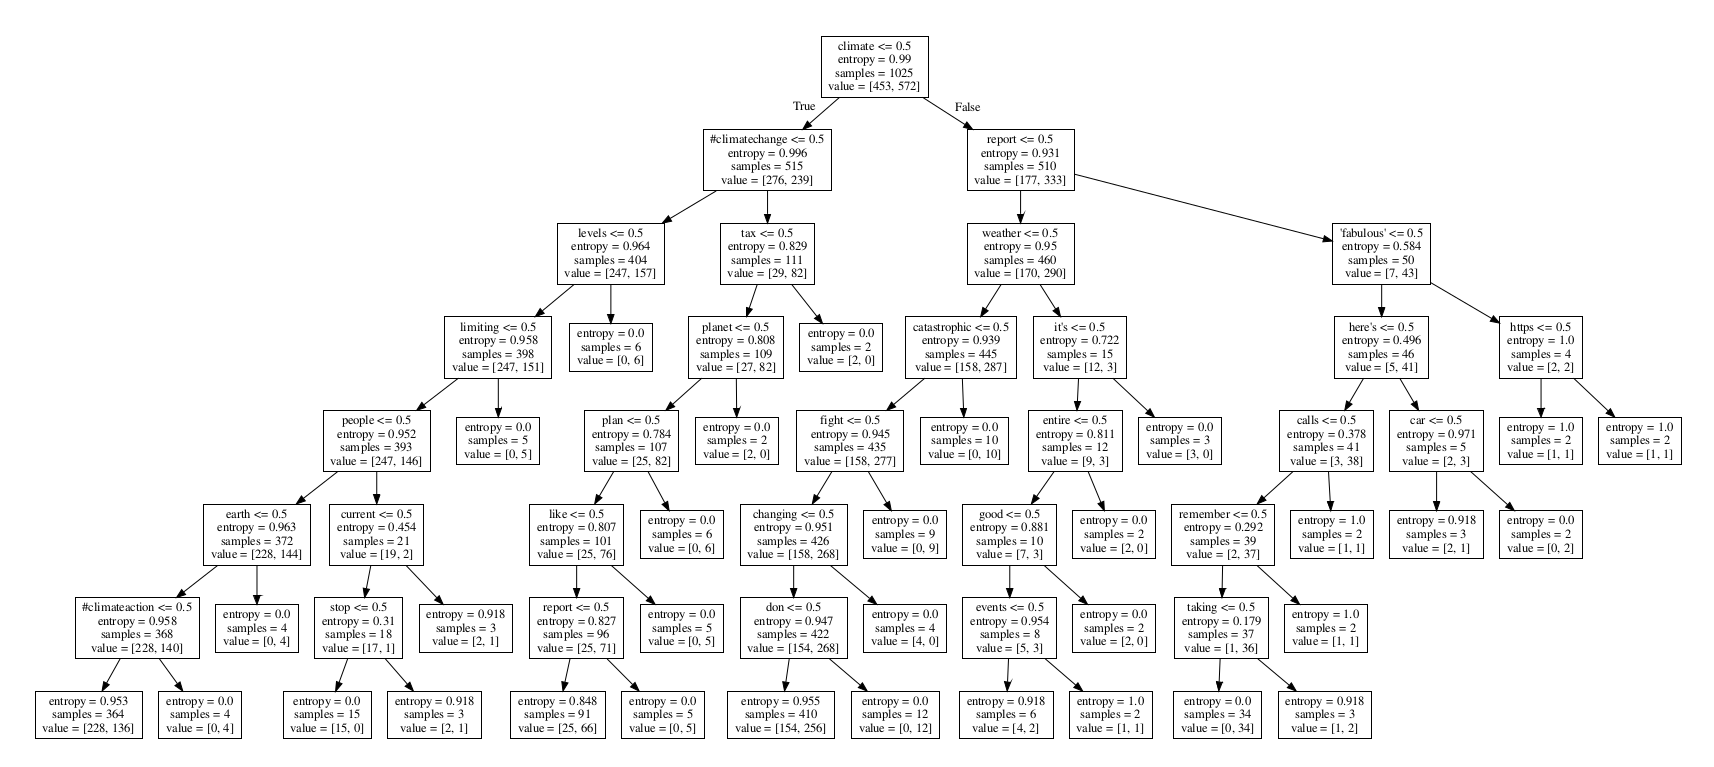
\includegraphics{1.png}
\caption{}
\end{figure}

\subsubsection*{Fold 2}\label{fold-2}

\begin{figure}[H]
\centering
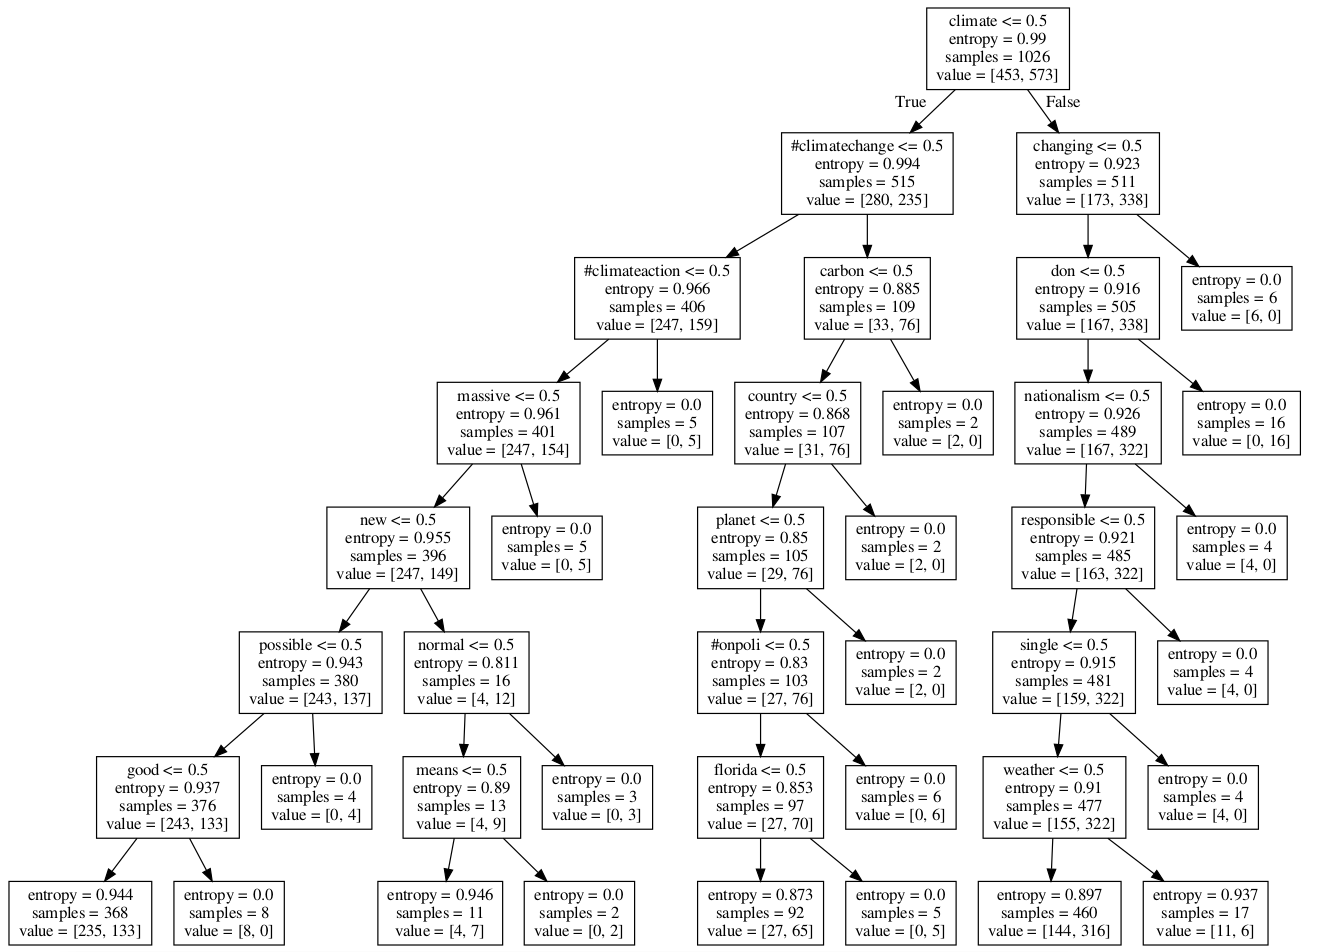
\includegraphics{2.png}
\caption{}
\end{figure}

\subsubsection*{Fold 3}\label{fold-3}

\begin{figure}[H]
\centering
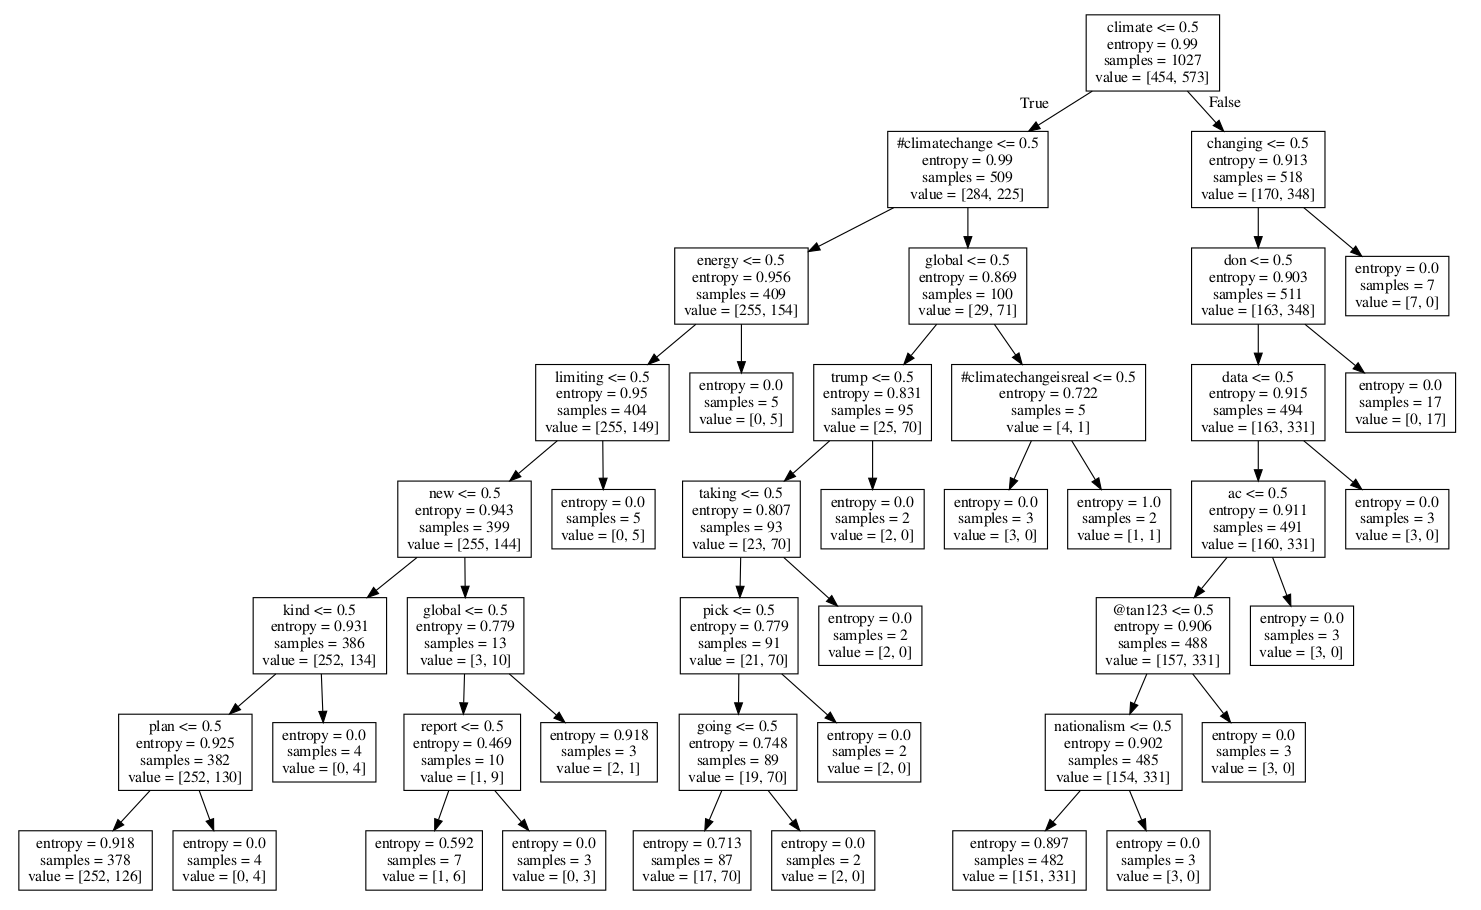
\includegraphics{3.png}
\caption{}
\end{figure}

\subsubsection*{Fold 4}\label{fold-4}

\begin{figure}[H]
\centering
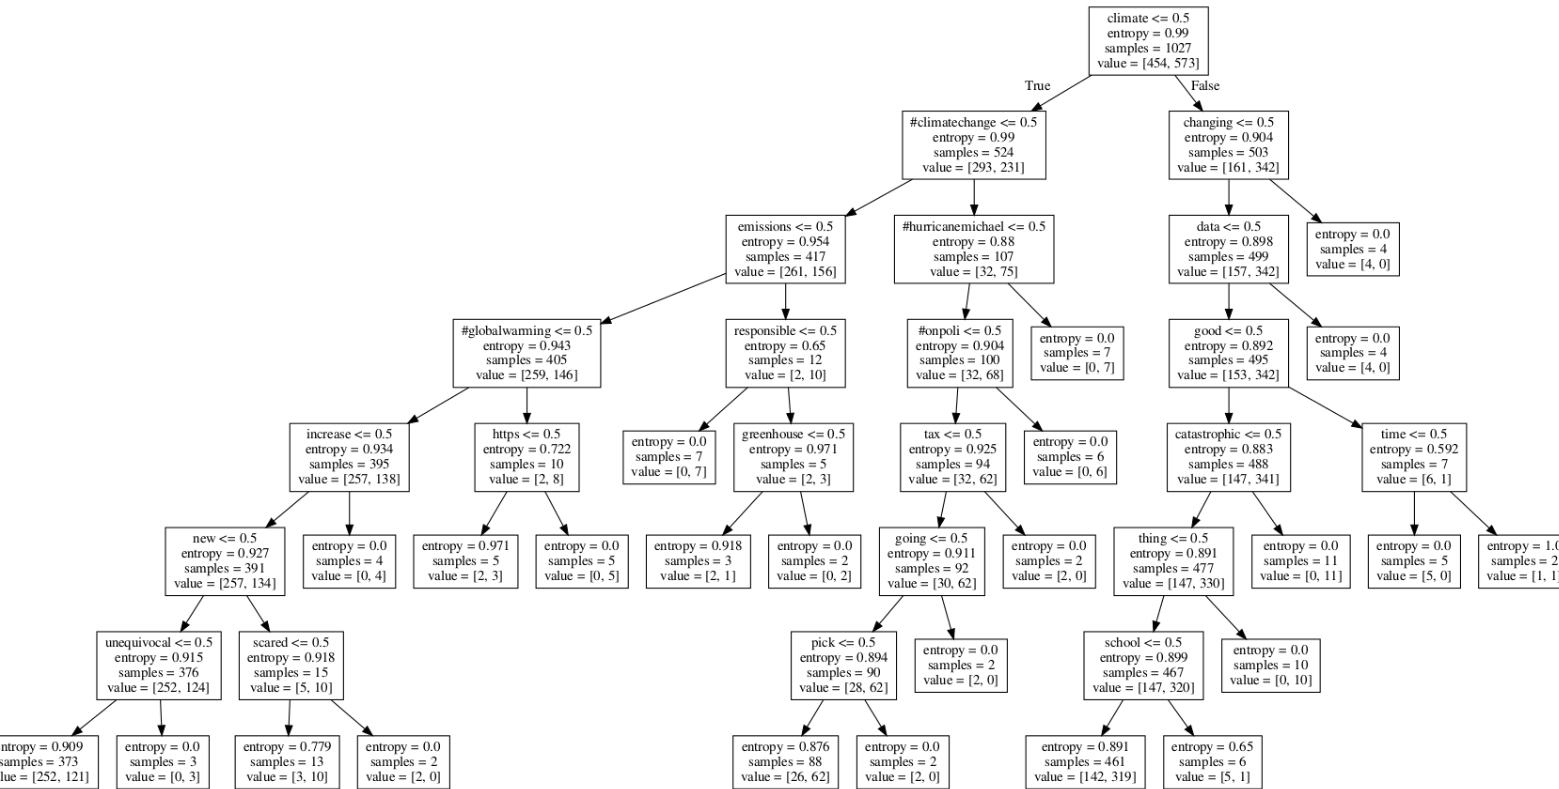
\includegraphics{4.png}
\caption{}
\end{figure}

\subsubsection*{Fold 5}\label{fold-5}

\begin{figure}[H]
\centering
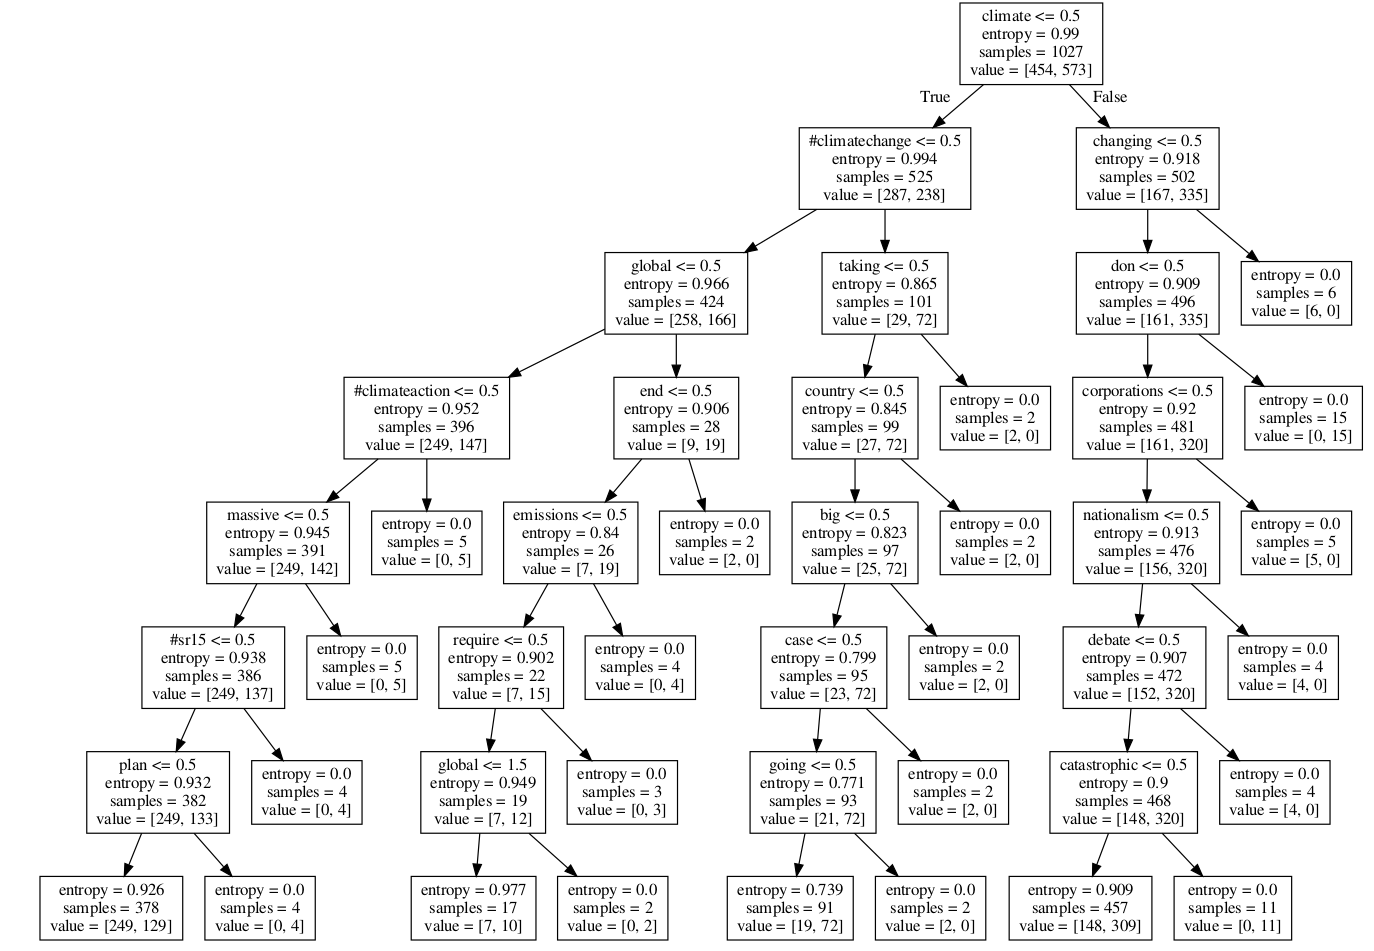
\includegraphics{5.png}
\caption{}
\end{figure}

    \subsubsection*{reload pickle}\label{reload-pickle}

    \begin{Verbatim}[commandchars=\\\{\}]
{\color{incolor}In [{\color{incolor}300}]:} \PY{n}{clf2} \PY{o}{=} \PY{n}{joblib}\PY{o}{.}\PY{n}{load}\PY{p}{(}\PY{l+s+s1}{\PYZsq{}}\PY{l+s+s1}{ClimateTeam7PD1.pkl}\PY{l+s+s1}{\PYZsq{}}\PY{p}{)}
          \PY{n}{y\PYZus{}pred} \PY{o}{=} \PY{n}{clf2}\PY{o}{.}\PY{n}{predict}\PY{p}{(}\PY{n}{X}\PY{p}{)}
          \PY{n}{f1\PYZus{}score}\PY{p}{(}\PY{n}{y}\PY{p}{,} \PY{n}{y\PYZus{}pred}\PY{p}{)}
\end{Verbatim}

\begin{Verbatim}[commandchars=\\\{\}]
{\color{outcolor}Out[{\color{outcolor}300}]:} 0.7355096602265155
\end{Verbatim}
            

    % Add a bibliography block to the postdoc
    
    
    
    \end{document}
